\chapter{Структура порождающей модели матрицы кросс-спектральной плотности.
         Подпространство протечки сигнала.} \label{chapt1}

% \section{Введение}
% План вводной части основного текста:
% Из чего мозг состоит и то, что электрические сигналы -- один из основных
% способов передачи инвормации между нейронами.
% В силу иерархичности системы информация передается не только от нейрона к нейрону,
% но и от популяции к популяциии. Ритмы мозга --- очень кратко.

% Есть гипотеза, что моменты коммуникации между популяциями сопровождаются когерентной
% активностью популяций. Есть и более сложные механизмы, нелинейной синхронизации,
% но они за пределами этого диссера.
% Что такой когерентность двух абстрактных сигналов (не про мозг).
% Зависимость от фазового угла мнимой и действительной части комплексной когерентности.
% Корреляция огибающей, коэффициент фазовой связности, Когерентность vs PLV для циркулярно-гауссовых сигналов.

% ЭЭГ и МЭГ как неинвазивный метод измерения электрической активности мозга.
% Пирамидальные клетки, их апикальные дендриты,
% пресинаптические\постсинаптические потенциалы, локальная синхронизация,
% токовый диполь, уравнения максвелла и их решение для диполя, топография
% и временная последовательность активации диполя, пару слов вращающемся диполе --
% просто как о модели, описывающей периодическое смещение активности,
% модель всего мозга, сетка объемная, сетка на коре, матрица прямой модели,
% топографии диполей как столбцы матрицы прямой модели и строки как поля
% чувствительности (lead fields), шум мозга и моделирование шума мозга. Модель ЭЭГ и МЭГ измерений
% X = GS + bn + b

Чтобы обрисовать контекст, в котором задача оценки коннективностей имеет смысл,
необходимо сперва описать основные принципы работы мозга, механизмы передачи
информации между нейронными популяциями и то, каким образом мы можем получить
информацию о таком обмене информацией средствами неинвазивной электрофизиологии.

Согласно оценкам~\ref{gorine}, в мозге здорового взрослого человека присутствует
порядка 83 миллиардов нейронов. Каждый отдельно взятый нейрон представляет собой
сравнительно простой биохимический механизм, принимающий электрические импульсы
от других нейронов на вход и способный генерировать выходной импульс в случае,
если входной сигнал превышает определенный порог. Тем не менее, этого элементарного
функционала отдельно взятых нейронов оказывается достаточно для обеспечения сложнейшей работы
головного мозга в целом.

Мозг, таким образом, представляет собой сложную систему, составленную из сравнительно
просто устроенных элементов.
По-прежнему неизвестно, за счет чего достигается
качественный скачок в поведении системы, состоящей из совокупности
нервных клеток, на пути от простой биоэлектрической сети,
узлы которой способны обмениваться электрическими импульсами, к
системе, обладающей интеллектом и сознанием собственного ``я''.
Каким-то образом оказывается возможен переход количества в качество, --- увеличение
числа сравнительно простых элементов системы,
таких как нейрон, до невероятных 83 миллиардов порождает удивительную
сложность и богатство поведенческих сценариев.

Тем не менее есть надежда, что ключ к пониманию работы мозга по крайней мере
частично лежит в изучении работы отдельных его частей и
способов обмена информацией между ними.

\section{Биологические механизмы обмена информацией между нейронными популяциями.}
Разберем сперва, какие именно механизмы позволяют нейронам обмениваться
электрическим сигналом на примере пирамидальных нейронов, из которых по
большей части и состоит кора больших полушарий.

Пирамидальный нейрон, как и любой другой, имеет аксон и
разветвленную сеть отростков, называемых дендритами.
Активность нейрона характеризуется генерацией так называемых
потенциалов действия или спайков в ответ на внешний электрохимический вход.

Потенциалы действия, распространяясь по аксону, достигают синапса.
Пришедший импульс играет роль триггера, провоцируя выделение
нейромедиаторов в  синаптическую щель. Нейромедиаторы достигают окончания
дендрита следующего нейрона, вызывая в нем увеличение, либо уменьшение
трансмембранного потенциала --- в зависимости от того, являлся
нейрон, сгенерировавший потенциал действия, тормозным или возбуждающим.
Трансмембранный потенциал определяется как разность потенциалов между
внешней и внутренней поверхностью мембраны клетки и зависит от молярных
концентраций ионов по обе стороны мембраны.
В такой схеме обмена информацей между двумя нейронами первый нейрон,
породивший потенциал действия, называется пресинаптическим, а второй,
принимающий сигнал --- постсинаптическим.

При этом, к каждому нейрону подведено множество аксонов.  Трансмембранный
потенциал отдельно взятого нейрона аккумулирует воздействия от нейронов, с
которыми у него имеются синаптические связи. Будучи равным $\approx -70$
микровольт в покое, трансмембранный потенциал изменяется в результате
потенциалов действия, приходящих от пресинаптических нейронов и, в при
достижении порога деполяризации мембраны в $\approx -30$ микровольт
постсинаптический нейрон сам производит потенциал действия.  Таким образом,
нейроны выполняют роль сумматоров в иерархической сети передачи сигнала.

Однако, прежде чем трансмембранный потенциал клетки ``почувствует'' изменения,
пришедший импульс должен через дендритные отростки достичь мембраны.
Электрический потенциал, распространяющийся по дендриту от синапса к мембране
носит название \emph{постсинаптического потенциала}. При этом, само
распространение электрической активности по дендриту есть ни что иное как
движение ионов, то есть электрический ток. На макроуровне совокупность нейронов
и окружающая их спинномозговая жидкость представляют собой объемный проводник,
из-за чего распространение токов вдоль дендритных отростков, называемых
\emph{первичными токами}, вызывает появление \emph{вторичных} объемных токов в
мозге.

Вследствие такой электрохимической проницаемости трансмембранные потенциалы
локальных нейронных популяций оказываются связаны между собой. В силу того, что
именно трансмембранный потенциал управляет генерацией потенциала действия, а
значит и передачей информации от нейрона к нейрону, оказывается, что отдельные
нейроны в информационном смысле не изолированы друг от друга, и можно говорить
о передаче информации не только от нейрона к нейрону, но и от популяции
нейронов к популяции.

Ключевой особенностью для работы групп пирамидальных нейронов является особая
организация их дендритных отростков, а именно --- наличие одного выделенного
дендрита, значительно превосходящего по размерам остальные. Такой дендрит
называется апикальным, а все остальные в рамках такой дихотомии --- базальными.

Пространственно апикальные дендриты пирамидальных нейронов в коре больших
полушарий организованы весьма особым образом --- если говорить о локальной
популяции, апикальные дендриты в ней ориентированы параллельно друг другу.
Вследствие этого первичные токи пирамидальных нейронов внутри популяции
суммируются, делая возможным их детектирование в неинвазивной
электрофизиологии. Действительно, электрическая активность отдельного нейрона
слишком слаба для регистрации за пределами черепной коробки существующими
сегодня методами, в то время как  суммарная активность групп из десятков тысяч
нейронов в силу коллинеарности их апикальных дендритов производит достаточный
ток для регистрации за пределами головы.
% TODO: какой ток? посмотри хамалайнена <22-01-18, yourname> %



Таким образом, обмен информацией между нейронами происходит посредством двух
основных механизмов~--- за счет распространения по аксону потенциала действия и
за счет распространения постсинаптических потенциалов, при чем оба эти
механизма тесно связаны между собой.

Одним из эпифеноменов такой взаимосвязи является появление в паттернах
суммарного постсинаптического потенциала ритмической осцилляторной активности
на сравнительно низких частотах.  Широко известен, например, альфа-ритм,
традиционно относимый к полосе частот $8-12$ Гц, с регистрации которого в 1924
году немецким физиологом Гансом Бергером ведет отсчет современная
электрофизиология.

Стоит отметить, что выделение отдельных полос частот из общего спектра
электрической активности групп нейронов неслучайно и связано с определенными
функциональными атрибутами, различными физиологически обусловленными причинами
их возникновения а также с их пространственной специфичностью.  Так, уже
упомянутый альфа-ритм в покое наиболее сильно представлен в затылочных долях
мозга и считается ритмом покоя зрительной коры в отсутствие визуального
раздражения.  К другим функционально-специфичным и широко освещенным в
литературе полосам частот относят дельта-, тета-, бета- и гамма-ритмы.

\subsection{Осцилляции и функциональная интеграция.}
Роль осцилляций в передаче информации между нейронными ансамблями на
сегодняшний день все еще остается плохо изученной, однако согласно доминирующей
в научном сообществе гипотезе взаимодействия через когерентность \ref{fries},
именно осцилляции постсинаптического потенциала являются медиатором
коммуникации между отдельными областями коры.

Такое взаимодействие предполагается необходимым в осуществлении так называемой
\emph{функциональной интеграции}. Суть понятия функциональной интеграции
состоит в следующем.

Известно, что существуют определенные зоны мозга, активность в которых
функционально специфична.  Так, например, было показано, что электрическая
стимуляция определенных областей прецентральной зоны провоцирует
неконтролируемые движения а иногда и активирует целые двигательные программы.
При этом в зависимости от конкретного места стимуляции задействуются различные
части тела.  Эти области прецентральной зоны принято называть первичной
моторной корой.  Оказыватся, что в первичной моторной коре представлена
подробная карта тела человека.  Аналогичная ситуация наблюдается и для
постцентральной зоны --- стимуляция соответствующих областей вызывает
тактильные ощущения в различных частях тела. Источник тактильного ощущения на
теле при этом также зависит от конкретного места стимуляции. В соответствии с
этим выделяют соматосенсорную кору. Такие функционально-специфичные зоны коры
существуют и для других отделов мозга. Тем не менее, не всякую активность
удается так хорошо локализовать на коре.

Так или иначе, субъективные ощущения подсказывают нам, что в реальной жизни
деятельность мозга никогда не сводится к какой-либо одной отдельно взятой
функции, как, скажем, движение указательным пальцем.  Скорее наоборот, большое
количество параллельных, но связанных друг с другом процессов осуществляется
мозгом одновременно. При этом для нормальной работы такие процессы должны
взаимодействовать друг с другом.  Для примера возьмем задачу в которой
испытуемому предлагали зажечь спичку, а затем проделать то же самое, но с
предварительной анастезией кончиков пальцев. Было показано, что потеря
чувствительности ведет к весьма значительному увеличению времени на выполнение
той же задачи.  Из этого можно заключить, что информация о тактильных ощущениях
определенным образом \emph{интегрируется} мозгом с двигательной программой при
выполнении задачи зажигания спички.

Термин \emph{функциональная интеграция} используется для обозначения такого
явления взаимодействия функционально-специфичных отделов мозга для решения
сложной когнитивной задачи, как в задаче со спичкой.  Предполагается, что раз
существуют зоны мозга, ответственные за осуществление той или иной функции, и
активные во время осуществления этой функции, то совместное осуществление
нескольких таких функций, требующих обмена информацией между собой должно
вызывать совместную активацию соответствующих областей мозга и обмен
информацией между ними.

\subsection{Взаимодействие через когерентность (гипотеза CTC).}

Теперь, введя понятие функциональной интеграции, мы можем вернуться к гипотезе
\emph{взаимодействия через когерентность}. Согласно этой гипотезе,
функциональная интеграция реализуется в мозге посредством установления
когерентных осцилляций постсинаптических потенциалов во взаимодействующих
областях коры.

% TODO: find paper on motor cortex and stimulation  <22-01-18, yourname> %
% TODO: find paper by sliman with dumb finger tips  <22-01-18, yourname> %

Обоснование гипотезы состоит в следующем.  Вероятность того, что нейрон
произведет потенциал действия тем больше, чем выше величина локального
постсинаптического потенциала. В силу того, что этот потенциал осциллирует,
нейрон способен реагировать на входящие потенциалы действия не всегда, а только
в те моменты, когда он был уже достаточно возбужден, т.е. тогда, когда
локальный постсинаптический потенциал находился в максимуме. Рассмотрим теперь
два нейрона, находящиеся в двух различных нейронных популяциях. Назовем первый
из них нейроном A, а второй --- нейроном B.  Для успешной передачи информации
от нейрона A к нейрону B необходимо, чтобы потенциал популяции нейрона B имел
достаточно высокое значение в тот момент, когда спайк от нейрона A достигнет
цели. Кроме того, чтобы нейрон A был способен произвести спайк, локальный
потенциал его популяции в момент генерации также должен быть достаточно высок.
Иными словами, осцилляции постсинаптического потенциала регулируют моменты
возможного приема и передачи информации между нейроном A и нейроном B. Таким
образом, возникает два временных окна, ритмически появляющихся и пропадающих во
времени --- первое окно соответствует промежуткам времени, когда нейрон A может
передать сигнал, а второе --- тем моментам времени, когда нейрон B может его
принять.  Если считать, что потенциал действия распространяется от аксона
нейрона A к дендриту нейрона B каждый раз за одно и то же время, то для
установления стабильного канала передачи информации от нейрона A к нейрону B
необходимо, чтобы эти два окна открывались и закрывались через одинаковые
промежутки времени, и чтобы окна приема информации было сдвинуто относительно
окна передачи на величину, равную времени распространения сигнала от нейрона A
к нейрону B.  Последнее справедливо в том случае, если осцилляции двух
нейронных популяций \emph{когерентны}, то есть имеют одинаковую частоту и,
возможно, некоторый ненулевой фазовый сдвиг.  Таким обзазом, согласно гипотезе
взаимодействия через когерентность, синхронизация осцилляций нейронных
популяций способствует обмену информацией в виде потенциалов действия между
ними, в то время как рассинхронизация осцилляций ведет к блокированию обмена
сигналами.


\subsection{Формальное определение когерентности}
Дадим более формальное определение когерентности абстрактных сигналов.
Пусть имеется два случайных процесса $s_1, s_2$:
\begin{equation}
    s_1 = s_1(t,\omega), s_2 = s_2(t,\omega)
\end{equation}
где переменная $t$~--- время, а $\omega$~--- случайная величина из
вероятностного пространства $\Omega$.  Под сигналами $s_1(t), s_2(t)$ будем
понимать конкретные реализации случайных процессов $s_1(t,\omega),
s_2(t,\omega)$, фиксируя величину $\omega = \omega_0$.

Наиболее естественным способом проверить, является ли один случайный процесс
сдвинутой во времени копией другого, является подсчет кросс-ковариации, которая
определяется как:

\begin{equation}
    C_{s_1, s_2}(t_1,t_2) = cov(s_1(t_1), s_2(t_2)) \defeq
    \Expect{(s_1(t_1,\omega) - \mu_1(t_1))(s_2(t_2,\omega) - \mu_2(t_2))}
    \label{eq:cross_covar_def}
\end{equation}
где $\mu_i(t_i) = E(s_i(t_i)), i=1,2$~--- среднее по ансамблю функции случайной величины величины
$s_i(t_i,\omega)$.

Для простоты изложения будем считать, что сигналы имеют нулевое среднее, имея в
виду, что мы всегда можем вычесть среднее по ансамблю из каждой реализации
случайного процесса.  Рассмотрим сначала случай стационарных в широком смысле
процессов, а потом обобщим рассуждения на случай нестационарности.
Стационарными в широком смысле называются такие случайные процессы, для которых
среднее не зависит от времени, а автоковариация зависит только от сдвигов по
времени.  Кроме того, мы потребуем от процессов \emph{совместной}
стационарности в широком смысле, то есть мы будем считать, что
кросс-ковариация, также зависит только от сдвига по времени $\tau = t_2 - t_1$:

\begin{equation}
    C_{s_1,s_2}(t_1,t_1+\tau) = C_{s_1,s_2}(\tau)
\end{equation}

Введем дополнительные понятия, которые понадобятся нам для определения
когерентности.  Сперва вспомним понятие энергии сигнала.  Энергией сигнала на
промежутке~$\Big[{-\frac{T}{2}},\frac{T}{2}\Big]$ называют величину

\begin{equation}
    E_T \defeq \Expect{\int\limits_{-T/2}^{+T/2} \abs{s(t,\omega)} ^ 2 dt}
\end{equation}

Полная энергия сигнала получается взятием предела от $E_T$:

\begin{equation}
    E \defeq \lim_{T \to \infty} E_T
\end{equation}

Для стационарных процессов, однако, величина полной энергии, вообще говоря, не
определена, поэтому вводят понятие средней мощности сигнала:

\begin{equation}
    P \defeq \lim_{T \to \infty}\frac{E_T}{T}
\end{equation}

Введем операцию преобразования Фурье на отрезке $\Big[{-\frac{T}{2}},\frac{T}{2}\Big]$
для процесса~$s$ следующим образом:

\begin{equation}
    F_s^T(f,\omega) \defeq \frac{1}{\sqrt{T}}\int\limits_{-T/2}^{T/2} s(t,\omega) e^{-ift} dt
\end{equation}

Тогда, пользуясь теоремой Парсеваля, для средней мощности сигнала будем иметь
\begin{equation}
    P = \lim_{T \to \infty} \Expect{\int\limits_{-\infty}^{+\infty}\abs{F_s^T(f,\omega)}^2df}
\end{equation}

Далее, определим спектральную плотность мощности сигнала:

\begin{equation}
    S_{ss}(f) \defeq \lim_{T \to \infty} \Expect{\abs{F_s^T(f,\omega)} ^ 2}
    \label{eq:psd_def}
\end{equation}

Спектральная плотность мощности характеризует распределение мощности сигнала по
частотам.  По аналогии с \ref{eq:psd_def} вводят понятие кросс-спектральной
плотности мощности

\begin{equation}
    S_{s_1,s_2}(f) \defeq \lim_{T \to \infty} \Expect{\conj{F_{s_1}^T(f,\omega)} F_{s_2}^T(f,\omega)}
    \label{eq:csp_def}
\end{equation}

Введя основные понятия, мы готовы теперь определить когеренцию и дать
интуитивное представление о том, почему величина когерентности отражает степень
синхронизации сигналов.

Для частотного образа функции кросс-ковариации случайных процессов,
стационарных в широком смысле, справедлива теорема Винера-Хинчина, согласно
которой кросс-ковариация и кросс-спектральная плотность мощности связаны друг с
другом через преобразование Фурье:

\begin{equation}
    S_{s_1, s_2}(f) = \int\limits_{-\infty}^{+\infty}C_{s_1,s_2}(\tau)e^{-if\tau}d\tau
\end{equation}

Или, используя \ref{eq:csp_def}:

\begin{equation}
    \lim_{T \to \infty} \Expect{\conj{F_{s_1}^T(f,\omega)} F_{s_2}^T(f,\omega)} =
    \int\limits_{-\infty}^{+\infty}C_{s_1,s_2}(\tau)e^{-if\tau}d\tau
\end{equation}

Рассмотрим подробнее, как устроено произведение
$\conj{F_{s_1}^T(f,\omega)} F_{s_2}^T(f,\omega)$.
Пользуясь экспоненциальным представлением комплексного числа, для коэффициента Фурье на частоте $f$
будем иметь:

\begin{equation}
    F_{s_j}^T(f) = A_j(f) * e^{i\phi_j}, j=\overline{1,2}
    \label{exp_fourier}
\end{equation}

где $A_i(f)$~--- амплитуда синусоиды на частоте $f$ в соответствующем
разложении Фурье, а $\phi_i$~--- ее фаза.  Отметим, что частотное представление
позволяет в явном виде получить доступ к фазе сигнала.

Используя \ref{exp_fourier}, можем переписать выражение для произведение фурье-образов
на отрезке $\Big[{-\frac{T}{2}}, \frac{T}{2}\Big]$ как:
\begin{equation}
    \conj{F_{s_1}^T(f,\omega)} F_{s_2}^T(f,\omega) =
    A_1(f,\omega)A_2(f,\omega) e^{i(\phi_2(f,\omega) - \phi_1(f,\omega))}
\end{equation}

Из соотношения выше видно, что на частоте $f$ фаза произведения фурье-образов
реализаций случайного процесса совпадает с разностью фаз соответствующих
комплексных экспонент для индивидуальных преобразований Фурье. Применяя далее
операцию усреднения по ансамблю, получим значение кросс-спектральной плотности
мощности на частоте $f$:

\begin{equation}
    S_{s_1, s_2}(f) = \Expect{A_1(f,\omega)A_2(f,\omega) e^{i(\phi_2(f,\omega) - \phi_1(f,\omega))}}
    \label{csp_exp}
\end{equation}

Таким образом, мы получили, что значение кросс-спектральной плотности мощности
равно среднему по ансамблю от комплексного числа, аргумент которого равен
разности фаз гармоник индивидуальных сигналов с частотой $f$, а  модуль~---
произведению амплитуд этих гармоник.  Имея в виду, что поле комплексных чисел
изоморфно двумерному векторному пространству, можем понимать операцию
усреднения в уравнении \ref{csp_exp} как усреднение векторов на плоскости,
повернутых относительно направления оси абсцисс на угол, равный разности фаз
сигналов.  Нетрудно понять, что средний вектор при фиксированных амплитудах
будет иметь тем большую норму, чем более воспроизводима соответствующая
разность фаз по реализациям случайного процесса.  Воспроизводимая по
реализациям разность фаз, в свою очередь, свидетельствует о синхронизации
случайных процессов, т.е. о наличии некой линейной связи между ними.  Таким
образом, длина результирующего вектора может служить мерой синхронности
случайных процессов.  Вместе с тем, чтобы исключить влияние амплитуды на
получающееся значение, применяют нормировку на среднее по ансамблю значение
мощностей сигналов на той же частоте.  Получающаяся нормированная величина и
есть по определению когерентность двух сигналов:

\begin{equation}
    G_{s_1,s_2}(f) \defeq \frac{S_{s_1,s_2}(f)}{\sqrt{S_{s_1,s_1}(f)S_{s_2,s_2}(f)}}
    \label{def_coh}
\end{equation}

Или, используя определение кросс-спектральной плотности мощности:

\begin{equation}
    G_{s_1,s_2}(f) = \lim_{T \to \infty}
    \frac{\Expect{\conj{F_{s_1}^T(f)}F_{s_2}^T(f)}}
    {\sqrt{\Expect{\conj{F_{s_1}^T(f)}F_{s_1}^T(f)}
    \Expect{\conj{F_{s_2}^T(f)}F_{s_2}^T(f)}}}
\end{equation}

Определенная таким образом функция когерентности может быть использована лишь
для стационарных в широком смысле сигналов.  В то же время предположение о
стационарности зачастую противоречит природе изучаемых процессов. В частности,
нестационарны по своей природе сигналы, возникающие в электрофизиологии.  Тем
не менее, возможно обобщить определение когерентности и на случай
нестационарности.  Обобщение достигается путем использования вместо
преобразования Фурье одного из \emph{частотно-временных преобразований}.  В
частности, можно использовать преобразование Фурье с окном,
вейвлет-преобразование или узкополосную фильтрацию с центральной частотой $f$ с
последующим извлечением аналитического сигнала.

В каждом из этих методов возникает характерная ширина временного окна (возможно
различная для разных частот $f$).  Предполагая, что статистические свойства
случайного процесса меняются со временем медленно, можем повторить рассуждения
выше для сужения стационарных процессов на временное окно частотно-временного
преобразования за исключением перехода, для которого мы использовали теорему
Винера-Хинчина.  Теорема Винера-Хинчина, однако, также допускает обобщение на
случай нестационарных процессов \ref{Paper2009}.

Таким образом, для нестационарных процессов будем иметь:

\begin{equation}
    G_{s_1,s_2}(f,t) \defeq
    \frac{\Expect{\conj{\mathcal{F}_{s_1}(f,t,\omega)}\mathcal{F}_{s_2}(f,t,\omega)}}
    {\sqrt{\Expect{\conj{\mathcal{F}_{s_1}(f,t,\omega)}\mathcal{F}_{s_1}(f,t,\omega)}
    \Expect{\conj{\mathcal{F}_{s_2}(f,t,\omega)}\mathcal{F}_{s_2}(f,t,\omega)}}}
    \label{nonwss_coh_def}
\end{equation}
где $\mathcal{F}_{s_i}(f,t,\omega)$~--- частотно-временной образ сигнала $s_i$ ($i=\overline{1,2}$)

Отметим одно интересное свойство функции когерентности.  Как в стационарном,
так и в нестационарном случае когерентность является комплекснозначной функцией
частоты $f$. При этом значения этой функции, согласно \ref{csp_exp},
пропорциональны средневзвешенной комплексной экспоненте с аргументом, зависящим
от разности фаз.  При этом веса равны произведениям амплитуд исходных сигналов
на заданной частоте.  Если в иллюстративных целях предположить, что амплитуды и
фазы независимы, получим для когерентности следующее выражение:

\begin{equation}
    G_{s_1,s_2}(f,t) =
    \frac{\Expect{A_1(f,t,\omega)A_2(f,t,\omega)}}
    {\sqrt{\Expect{A_1(f,t,\omega)^2}\Expect{A_2(f,t,\omega)^2}}}\Expect{e^{i\Delta\phi(f,t,\omega)}},
\end{equation}

где $\Delta\phi = \phi_2 - \phi_1$. Рассмотрим подробнее множитель
$\Expect{e^{i\Delta\phi(f,t,\omega)}}$.  В случае, если разность фаз
$\Delta\phi$ от реализации к реализации будет иметь воспроизводимые близкие к
нулю значения, средняя комплексная экспонента также будет иметь близкий к нулю
аргумент, т.е. действительная часть результирующей комплексной экспоненты будет
иметь высокое значение по сравнению с мнимой частью.  Иными словами, если
случайные процессы были синхронизированы с нулевой фазой, их функция
когерентности будет иметь почти действительные значения. С другой стороны, если
разность фаз воспроизводимо близка к $\pi/2$, итоговое значение когерентности
будет близко к мнимому числу.  Это наблюдение понадобится нам в дальнейшем, так
как одной из наиболее популярных сегодня методик оценки коннективности на
неинвазивных данных является так называемая мнимая часть когерентности.

% PLV vs coh {{{plv %
% Тем не менее, предположение о независимости амплитуд и фаз сигналов вообще говоря неверно.
% Кроме того, амплитуды двух сигналов могут быть также коррелированы, что приводит к определенным
% затруднениям при интерпретации результатов анализа, полученных на основе рассчета когерентности.

% Чтобы исключить влияние амплитуд на оценку фазовой связности случайных процессов,
% была предложена мера, получившая название ``коэффициент фазовой связности'' (phase locking value, PLV) \ref{PLV},
% которая определяется как

% \begin{equation}
%     PLV_{s_1,s_2}(f,t) \defeq \abs{\Expect{e^{i\Delta\phi(f,t,\omega)}}}
% \end{equation}

% Или, через образы частотно-временных преобразований:

% \begin{equation}
%     PLV_{s_1,s_2}(f,t) = \Expect{\frac{\conj{\mathcal{F}_{s_1}(f,t,\omega)}\mathcal{F}_{s_2}(f,t,\omega)}
%     {\abs{\mathcal{F}_{s_1}(f,t,\omega)}\abs{\mathcal{F}_{s_2}(f,t,\omega)}}}
% \end{equation}
% plv}}} %

\section{Модель неинвазивных МЭГ/ЭЭГ измерений.}

В предыдущих разделах мы рассмотрели, каким образом установление когерентных
осцилляций между постсинаптическими потенциалами нейронных популяций позволяет
осуществлять функциональную интеграцию, а также сделали первый шаг на пути к
оценке когерентности на основании измерений электрической активности мозга~---
дали формальное определение функции когерентности двух случайных процессов.

В определении когерентности \ref{def_coh} фактически содержится рецепт ее
вычисления --- нам лишь необходимо оценить значения соответствующих мат.
ожиданий из данных.

Однако в неинвазивной электрофизиологии мы не имеем прямого доступа к локальным
осцилляциям потенциалов в нейронных популяциях, так как активность мозга
регистрируется при помощи сенсоров, находящихся за пределами головы и
следовательно отражает некую суммарную активацию нейронных ансамблей.

Как было отмечено выше, источником сигнала, снимаемого при помощи ЭЭГ или МЭГ
служат первичные токи, т.е. токи, распространяющиеся вдоль апикальных дендритов
пирамидальных нейронов коры.  Первичные токи вызывают появление вторичных токов
в объемном проводнике, которым является мозг.  В силу параллельной ориентации
апикальных дендритов, электромагнитные поля, порождаемые первичными токами,
накладываются, генерируя суммарное электрическое поле достаточной силы для
регистрации за пределами головы.

Чтобы понять, как соотносятся суммарные колебания постсинаптического
потенциала, порождаемые нейронными популяциями, с регистрируемым сигналом,
начнем с рассмотрения уравнений Максвелла.

\subsection{Уравнения Максвелла в квазистатическом приближении.}
% (выкладки ниже приведены на основе
% статьи \cite{Hamalainen1993}):

В общем виде для проводящей среды уравнения Максвелла можно записать в виде

\begin{gather}
    \nabla \cdot \mathbf{E}  = \frac{\rho}{\epsilon_0} \label{eq:max1} \\
    \nabla \times \mathbf{E} = {-\frac{\partial \mathbf{B}}{\partial t}} \label{eq:max2} \\
    \nabla \cdot \mathbf{B}  = 0 \label{eq:max3} \\
    \nabla \times \mathbf{B} = \mu_0 (\mathbf{J} + \epsilon_0 \frac{\partial \mathbf{E}}{\partial t})
    \label{eq:max4},
\end{gather}
где $\mathbf{E}$~--- напряженность электрического поля, $\mathbf{B}$~--- магнитная индукция,
$\rho$~--- объемная плотность стороннего электрического заряда,
$\mathbf{J}$~--- плотность электрического тока,
$\mu_0$~--- магнитная постоянная,
$\epsilon_0$~--- электрическая постоянная.



При этом для мозга магнитная проницаемость $\mu = \mu_0$.  В немагнитной среде
без диспесии $\mathbf{J}$ является суммой омических и поляризационных токов:

\begin{equation}
    \mathbf{J} = \sigma \mathbf{E} + \frac{\partial \mathbf{P}}{\partial t},
    \label{eq:current_in_nonmagnetic}
\end{equation}
где $\mathbf{P} = (\epsilon - \epsilon_0) \mathbf{E}$ --- вектор поляризации,
а $\epsilon$ --- диэлектрическая проницаемость среды.

В электрофизиологии принято рассматривать уравнения  Максвелла квазистатическом
приближении, которое заключается в том, что в уравнениях выше мы можем опустить
производные напряженности электрического поля и магнитной индукции по времени
($\frac{\partial \mathbf{E}}{\partial t}$ и $\frac{\partial
\mathbf{B}}{\partial t}$).  Дело в том, что в нейромагнетизме мы как правило
имеем дело с частотами колебаний $\leq 100$ Гц; на клеточном уровне
электрохимические процессы по большей части происходят на частотах менее 1000
кГц.  Таким образом, для электрического процесса, проходящего на частоте $f$,
будем иметь

\begin{equation}
    \mathbf{E} = \mathbf{E}_0 e^{i2\pi ft}
\end{equation}

Рассматривая теперь уравнения~\ref{eq:max4},~\ref{eq:current_in_nonmagnetic}, будем иметь:

\begin{equation}
    \nabla \times \mathbf{B} = \mu_0 (\sigma E +
    (\epsilon - \epsilon_0) \frac{\partial \mathbf{E}}{\partial t} +
    \epsilon_0 \frac{\partial \mathbf{E}}{\partial t}),
\end{equation}

Квазистатическое приближение уравнений Максвелла справедливо в том случае, если
члены в уравнении выше, содержащие производные по времени, малы по сравнению с
омическими токами: $\abs{\epsilon \frac{\partial \mathbf{E}}{\partial t}} \ll
\abs{\sigma \mathbf{E}}$, то есть если $2\pi f \epsilon / \sigma \ll 1$.

Полагая $\sigma = 0.3\;\text{Ом}^{-1} \cdot \text{м}^{-1}$  (значение для
тканей мозга), $\epsilon = 10^5\epsilon_0$, а $f =  100\;\text{Гц}$, получим
$2\pi f \epsilon / \sigma = 2 \times 10^{-3} \ll 1$.

Кроме того, значение $\frac{\partial \mathbf{B}}{\partial t}$ также должно быть
мало.  Из уравнений \ref{eq:max2} и \ref{eq:max4} будем иметь:

\begin{equation}
    \nabla \times \nabla \times \mathbf{E} =
    - \frac{\partial}{\partial t} (\nabla \times \mathbf{B}) =
    - \mu_o \frac{\partial}{\partial t}(\sigma \mathbf{E} + \epsilon \frac{\partial \mathbf{E}}{\partial t}) =
    - i 2\pi f \mu_0 (\sigma + i 2\pi f \epsilon) \mathbf{E}
\end{equation}

Для решений этого уравнения характерный пространственный масштаб имеет величину

\begin{equation}
    \lambda_c = \abs{2\pi f \mu_0 \sigma (1 + 2\pi f \epsilon / \sigma)}^{-1/2}.
\end{equation}

Для значений параметров, указанных выше, $\lambda_c  = 65 \text{м}$ и
значительно превосходит диаметр головы. Следовательно, можем пренебречь вкладом
члена $\frac{\partial \mathbf{B}}{\partial t}$ в значение величины
$\mathbf{E}$.

В квазистатическом приближении $\nabla \times \mathbf{E} = 0$, а значит
напряженность электрического поля представима в виде скалярного потенциала

\begin{equation}
    \mathbf{E} = - \nabla V
    \label{eq:scal_pot}
\end{equation}

Окончательно в квазистатическом приближении система уравнений Максвелла перепишется в виде:

\begin{gather}
    \Laplace V = -\frac{\rho}{\epsilon_0} \label{eq:max_quasi1} \\
    \nabla \cdot \mathbf{B} = 0 \label{eq:max_quasi2} \\
    \nabla \times \mathbf{B} = \mu_0 \mathbf{J} \label{eq:max_quasi3},
\end{gather}

\subsection{Первичные и вторичные токи.}
Рассмотрим теперь, как первичные и вторичные токи входят в уравнения Максвелла.
Из уравнений выше видно, что объемная плотность тока $\mathbf{J}(\mathbf{r})$
представима в виде суммы двух компонент. Объемные омические токи
$\mathbf{J}^v(\mathbf{r}) = \sigma(\mathbf{r}) \mathbf{E}(\mathbf{r})$ по своей
физической природе пассивны и появляются в следствие действия макроскопического
электрического поля на носистели заряда в проводящей среде.  Эти токи мы будем
называть \emph{вторичными}.  Остальные члены уравнения будем относить к
\emph{первичным} токам $\mathbf{J}^p$:

\begin{equation}
    \mathbf{J}(\mathbf{r}) =
    \mathbf{J}^p(\mathbf{r}) + \sigma(\mathbf{r}) \mathbf{E}(\mathbf{r}) =
    \mathbf{J}^p(\mathbf{r}) - \sigma(\mathbf{r}) \nabla V(\mathbf{r})
    \label{eq:prim_sec_cur}
\end{equation}

Такое определение не имело бы смысла без указания соответствующего
пространственного масштаба.  Здесь $\sigma(\mathbf{r})$ --- макроскопическая
проводимость; детали, относящиеся к клеточному масштабу, мы оставляем без
внимания. Иными словами, весь объем мозга моделируется как однородный объемный
проводник.  Разделение в уравнении \ref{eq:prim_sec_cur} иллюстрирует тот факт,
что нейрональная активность порождает первичные токи по большей части вблизи
клетки, тогда как вторичные токи протекают повсюду в объеме проводящей среды.
Таким образом, найдя источники первичных токов, мы найдем источники
нейрональной активности мозга.

Необходимо дополнительно отметить, что источники токов $\mathbf{J}^p$ должны
рассматриваться как батарейки, помещенные в макроскопический проводник. При
этом, хотя преобразование градиентов концентраций в ток происходит в основном
благодаря диффузии, первичные токи во многом определяются структурой
проводимости на клеточном уровне. В частности, клеточные мембраны, будучи
хорошим проводником, определяют направление как внутриклеточных, так и
межклеточных токов.

Перепишем уравнения Максвелла с учетом разделения на первичные и вторичные токи:
\begin{gather}
    \Laplace V = -\frac{\rho}{\epsilon_0} \label{eq:max_quasi_prim_sec1} \\
    \nabla \cdot \mathbf{B} = 0 \label{eq:max_quasi_prim_sec2} \\
    \nabla \times \mathbf{B} = \mu_0 (\mathbf{J}^p - \sigma \nabla V) \label{eq:max_quasi_prim_sec3},
\end{gather}

\subsection{Модель токового диполя.}

Итак, для определения истчников нейрональной активности на коре необходимо
локализовать источники первичных токов.

По существующим оценкам, минимальное количество пирамидальных нейронов,
необходимое для создания измеримого за пределами головы поля для МЭГ составляет
$\approx$

% TODO: find in Hamalainen <01-02-18, yourname> %
А для ЭЭГ ---
% TODO: lookup somewhere  <01-02-18, yourname> %

При этом размер участка коры, соответствующий такому количеству нейронов
составляет ???, а источник и сток заряженных частиц разнесены на расстояние
порядка ???. По отношению к характерному расстоянию до сенсоров размеры
локальных источников суммарного тока малы и могут считаться точечными.  Для
моделирования таких точечных источников тока на коре вводят понятие
\emph{токового диполя}.

Под токовым диполем понимают такой источник тока, у которого сток и исток
разнесены на пренебрежимо малое расстояние.  Токовый диполь характеризуется
тремя координатами, задающими его положение в пространстве, а также дипольным
моментом~--- вектором, характеризующим величину и направление тока.

% При численном моделировании для дискретизации пространства всех возможных источиков
% первичных токов пользуются аппроксимацией первичных токов \emph{токовыми диполями}.
Токовый диполь $\mathbf{Q}$ в точке $\mathbf{r}_Q$ можно представить себе как сосредоточенный
в одной точке источник первичного тока:
\begin{equation}
    \mathbf{J}^p(\mathbf{r}) \defeq \mathbf{Q}\delta(\mathbf{r} - \mathbf{r}_Q),
    \label{eq:cur_dip_def}
\end{equation}
где $\delta(\mathbf{r})$~--- дельта-функция Дирака.
В МЭГ/ЭЭГ приложениях токовые диполи используют в качестве эквивалентных источников первичных токов для
участков коры по площади иногда доходящих до нескольких квадратных сантиметров.

В силу линейности уравнений Максвелла активность распределенного по коре набора токовых
диполей отобразится на сенсорах как суперпозиция активностей отдельных диполей, поэтому
для построения модели данных, записываемых в МЭГ/ЭЭГ парадигме,
рассмотрим, как выглядит за пределами головы электромагнитная активность отдельного токового диполя.

\subsection{Поиск решений для кусочно постоянного профиля проводимости.}
Для определения магнитного поля за пределами головы проинтегрируем уравнение~\ref{eq:max_quasi_prim_sec3}:
\begin{equation}
    \mathbf{B}(\mathbf{r}) = \frac{\mu_0}{4\pi}\int \limits_{G} (\mathbf{J}^p(\mathbf{r}^\prime) -
    \sigma(\mathbf{r}') \nabla V(\mathbf{r}')) \times \frac{\mathbf{R}}{R^3} dv'
    \label{eq:B_integral}
\end{equation}

Здесь $\mathbf{R} = \mathbf{r} - \mathbf{r}'$~--- расстояние от источника тока до точки,
в которой мы хотим определить значение вектора магнитной индукции.
При этом мы предполагаем, что за пределами головы источники первичных токов отсутствуют,
а проводимость равна нулю, поэтому объемный интеграл в уравнении \ref{eq:B_integral}
берется не по бесконечной области, а лишь по объему головы $G$.

Заметим, что $\sigma(\mathbf{r}')$ вообще говоря различна для разных точек головы.
Тем не менее, в объеме головы можно выделить области однородной проводимости, такие как
кожа головы, череп, цереброспинальная жидкость, серое и белое вещество.
Будем считать, что в объеме головы содержится $m$ таких областей, которые мы обозначим как $G_i$.
Тогда уравнение \ref{eq:B_integral} перепишется в виде:

\begin{equation}
    \mathbf{B}(\mathbf{r}) = \mathbf{B}_0(\mathbf{r}) -
\frac{\mu_0}{4\pi}\sum_{i=1}^{m}\sigma_i \int \limits_{G_i} \nabla V(\mathbf{r}')
\times \frac{\mathbf{R}}{R^3} dv',
    \label{eq:B_integral_1}
\end{equation}
где
\begin{equation}
    \mathbf{B}_0(\mathbf{r}) =
    \frac{\mu_0}{4\pi}\int \limits_{G} \mathbf{J}^p(\mathbf{r}') \times \frac{\mathbf{R}}{R^3} dv'
    \label{eq:B_0_def}
\end{equation}
представляет собой магнитное поле, порождаемое только первичными токами.

Далее, используя векторное равенство $\nabla \times (V \nabla(1/R)) = \nabla V \times \nabla (1/R)$
и $\int \limits_{G} \nabla \times \mathbf{u} dv = \int \limits_{S} \mathbf{S}\times\mathbf{u}$
получим
\begin{equation}
    \int \limits_{G_i} \nabla' V \times \frac{\mathbf{R}}{R^3} dv' =
    \int\limits_{G_i} \nabla' V \times \nabla' \frac{1}{R} dv' =
    - \int \limits_{\partial G_i} V \nabla' \frac{1}{R} \times \mathbf{dS}'
\end{equation}
Здесь $d\mathbf{S}' = \mathbf{n}(\mathbf{r}') dS'$; $\mathbf{n}(\mathbf{r}')$ ---
вектор внешней нормали к границе $i$-той области $\partial G_i$. Комбинируя слагаемые на каждой границе $S_{ij}$,
получим
\begin{equation}
        \mathbf{B}(\mathbf{r}) = \mathbf{B}_0(\mathbf{r}) -
        \frac{\mu_0}{4\pi}\sideset{}{'}\sum_{i,j}(\sigma_i - \sigma_j) \int \limits_{S_{ij}} V(\mathbf{r}')
        \frac{\mathbf{R}}{R^3} \times \mathbf{dS}'_{ij}
        \label{eq:B_surf}
\end{equation}

Из этого уравнения легко увидеть, что при расчете магнитного поля  объемные токи могут быть
заменены эквивалентными поверхностными токами
$-(\sigma_i - \sigma_j) V(\mathbf{r}')\mathbf{n}_{ij}(\mathbf{r}')$
на каждой из границ между областями однородной проводимости $S_{ij}$.

Чтобы получить $\mathbf{B}$ из уравнения \ref{eq:B_surf}, необходимо знать значения $V$ на $S_{ij}$.
Пользуясь теоремой Грина $\int\limits_{G}(\phi\nabla^2\psi - \psi\nabla^2\phi)dv = \int\limits_{S}(\phi\nabla\psi-\psi\nabla\phi)\cdot \mathbf{dS}$, получим:

\begin{multline}
    \sum_{i=1}^m\sigma_i\int\limits_{G_i} \bigg[\frac{1}{R} \nabla'^2V - V\nabla'^2 \frac{1}{R}\bigg]dv'=\\
    = \sideset{}{'}\sum_{ij}\int\limits_{S_{ij}}\Bigg[\sigma_i\bigg[\frac{1}{R}\nabla'_iV -
        V\nabla'\frac{1}{R}\bigg] - \sigma_j \bigg[\frac{1}{R}\nabla'_j V - V \nabla'\frac{1}{R}\Bigg]
        \cdot\mathbf{dS}'_{ij}
        \label{eq:V_green}
\end{multline}


Здесь $\nabla'_i$ обозначает взятие градиента на границе внутри области с индексом $i$.
Так как плотность тока $\sigma\nabla V \cdot \mathbf{n}$ непрерывна на $S_{ij}$, правая часть уравнения
\ref{eq:V_green} приводится к

\begin{equation}
    {-\sideset{}{'}\sum_{ij}(\sigma_i - \sigma_j)}
\int\limits_{S_{ij}} V\nabla'\frac{1}{R}\cdot\mathbf{dS}'_{ij}
\end{equation}

Для преобразования левой части уравнения сначала применим оператор дивергенции
к уравнению~\ref{eq:prim_sec_cur}:
\begin{equation}
    \nabla \cdot \mathbf{J}^p = \nabla \cdot \mathbf{J} + \nabla \cdot(\sigma\nabla V)
\end{equation}

Далее, используя уравнение \ref{eq:max_quasi3} и тот факт, что дивергенция ротора равна нулю,
получим, что для квазистатического приближения $\nabla \cdot \mathbf{J} = 0$, а значит:
\begin{equation}
    \nabla\cdot(\sigma\nabla V) = \nabla \cdot \mathbf{J}^p
    \label{eq:18}
\end{equation}

Теперь, используя для левой части уравнения~\ref{eq:V_green} уравнение~\ref{eq:18}, а также равенство~
${\nabla'}^2\frac{1}{R} = {-4\pi\delta(\mathbf{R})}$, получим:
\begin{equation}
    V(\mathbf{r})\sigma(\mathbf{r}) = \sigma_0V_0(\mathbf{r}) -
    \frac{1}{4\pi}\sideset{}{'}\sum_{ij}(\sigma_i - \sigma_j)
    \int \limits_{S_{ij}}V(\mathbf{r}')\frac{\mathbf{R}}{R^3}\cdot \mathbf{dS}'_{ij}
\end{equation}
где
\begin{equation}
    V_0(\mathbf{r}) =
    {-\frac{1}{4\pi\sigma_0}\int\limits_{G}\mathbf{J}^p(\mathbf{r}')\cdot\nabla'\frac{1}{R}dv'} =
    \frac{1}{4\pi\sigma_0} \int\limits_{G}\frac{\nabla'\cdot \mathbf{J}^p}{R} dv'
\end{equation}

Чтобы получить интегральное уравнение для величины $V$ на поверхностях $S_{ij}$, устремим
$\mathbf{r}$ к точке на поверхности $S_{ij}$. Используя предельное значение \cite{vladimirov}
\begin{equation}
    \lim_{\mathbf{r}_0 \to \mathbf{r} \in S_{ij}}
    \int \limits_{S_{ij}} V(\mathbf{r}')
    \frac{\mathbf{r}_0-\mathbf{r}'}{\abs{\mathbf{r}_0 - \mathbf{r}'}^3} \cdot \mathbf{dS}_{ij}
        = {-2\pi V(\mathbf{r}) + \int \limits_{S_{ij}}V(r')\frac{\mathbf{R}}{R^3}\cdot \mathbf{dS}'_{ij}}
\end{equation}

получим итегральное уравнение для $V(\mathbf{r})$:
\begin{equation}
    (\sigma_i + \sigma_j) V(\mathbf{r}) = 2\sigma_0V_0(\mathbf{r}) + \frac{1}{2\pi} \sideset{}{'}\sum_{ij}
    \int \limits_{S_{ij}} V(\mathbf{r}')d\Omega_r(\mathbf{r}')
    \label{eq:V_surf}
\end{equation}

где $\mathbf{r} \in S_{ij}$, а $d\Omega_r(\mathbf{r}') =
{-\abs{\mathbf{r}-\mathbf{r}'}^{-3}(\mathbf{r}-\mathbf{r}')\cdot \mathbf{dS}'_{ij}}$~---телесный угол,
под которым дифференциальный элемент поверхности $\mathbf{dS}_{ij}$
в точке $\mathbf{r}'$ виден из точки $\mathbf{r}$.

Соотношение выше представляет собой линейное интегральное уравнение
на величину потенциала электрического поля $\sigma(\mathbf{r})$
на поверхностях разрыва функции $\sigma(\mathbf{r})$.
Одной из таких поверхностей является, в частности, поверхность кожи головы,
на которой мы меряем разность потенциалов при записи ЭЭГ.
Таким образом, уравнение~\ref{eq:V_surf} позволяет нам получить модель данных для ЭЭГ измерений.
Кроме того, восстановив значения потенциала $V$ на поверхностях $S_{ij}$
и подставив их в уравнение~\ref{eq:B_surf},
можем найти значение вектора магнитной индукции за пределами головы,
вследствие чего получим модель измерений для МЭГ.

В общем случае уравнения~\ref{eq:B_surf} и~\ref{eq:V_surf} нужно решать численно, однако оказывается,
что для уравнения~\ref{eq:B_surf} описывающего поведение вектора магнитной индукции,
возможно дополнительное упрощение,
позволяющее получить аналитическое выражение для неизвестной величины $\mathbf{B}(\mathbf{r})$.
Суть упрощающего предположения состоит в том, что объем головы приближенно полагается сферой.

\subsection{Случай сферически симметричного проводника.}
Рассмотрим уравнение~\ref{eq:B_surf} для сферически-симметричного проводника.
Для простоты  предположим, что начало координат совпадает с центром симметрии сферы,
аппроксимирующей объем головы.
Во-первых, заметим, что радиальная компонента вектора магнитной индукции
$B_r = \mathbf{B}(\mathbf{r}) \mathbf{e}_r = \mathbf{B}(\mathbf{r})\frac{\mathbf{r}}{\abs{\mathbf{r}}}$
не чувствительна к вторичным токам, так как

\begin{equation}
    (\mathbf{r} - \mathbf{r}') \times n(\mathbf{r}') \cdot \mathbf{e}_r =
    (\mathbf{r}-\mathbf{r}') \times
    \frac{\mathbf{r}'}{\abs{\mathbf{r}'}}\cdot\frac{\mathbf{r}}{\abs{\mathbf{r}}} = 0
\end{equation}

Следовательно, радиальная компонента вектора магнитной индукции может быть рассчитана из
уравнения~\ref{eq:B_integral} простой заменой $\mathbf{J}$ на $\mathbf{J}^p$:

\begin{equation}
    B_r = {-\frac{\mu_0}{4\pi}\int \mathbf{J}^p(\mathbf{r}')
    \times \frac{\mathbf{R}}{R^3}\cdot \mathbf{e}_r dv'}
    \label{eq:B_sphere_int}
\end{equation}


Для источников, имеющих вид токового диполя соотношение для определения вектора магнитной индукции
за пределами головы приобретает совсем простой вид:
\begin{equation}
    B_r = {-\frac{\mu_0}{4\pi}
    \frac{\mathbf{Q} \times \mathbf{r}_Q \cdot \mathbf{e}_r}
         {\abs{\mathbf{r} - \mathbf{r}_Q}^3}}
\end{equation}

Кроме того, так как $\nabla \mathbf{B} = 0$ за пределами проводника, значение величины $\mathbf{B}$
может быть получено из величины скалярного потенциала $\mathbf{B} = {-\mu_0 \nabla U}$.
Так как $\nabla \cdot \mathbf{B} = 0$, $U$ --- гармоническая функция и следовательно может быть однозначно
восстановлена по своей нормальной производной на границе проводника при условии, что она обращается
в ноль на бесконечности. Для сферы нормальная производная $\partial U / \partial \mathbf{r} = {-B_r / \mu_0}$.
Проинтегрировав это соотношение, получим:

\begin{equation}
    U(\mathbf{r}) = \frac{1}{\mu_0} \int \limits_{t=1}^{\infty} B_r(t\mathbf{r})dt
\end{equation}

Таким образом, в случае сферической симметрии проводника, зная радиальную компоненту вектора
магнитной индукции мы можем восстановить скалярный потенциал $U$, а значит и весь вектор $\mathbf{B}$.
Иными словами, для сферически симметричного проводника магнитное поле за его пределами
целиком определяется его радиальной компонентой $B_r$.

Отметим одно важное следствие соотношения~\ref{eq:B_sphere_int}. В случае когда первичный ток имеет
радиальное направление, $\mathbf{J}^p = J^p(\mathbf{r}') \mathbf{r}'/\abs{\mathbf{r}'}$,
$B_r$ становится равным нулю. Из $B_r=0$ следует $U = 0$, а значит и $\mathbf{B}=0$.
Это соотношение остается справедливым для любого осесимметричного тока в осесимметричном проводнике.
Кроме того, если источник первичного тока находится в центре сферы $B_r$ также
будет равно нулю в силу $\mathbf{r}_Q = 0$. Вообще, чем ближе источник первичного тока к центру сферы,
тем меньше вклад от него в суммарное магнитное поле за пределами проводника.

Таким образом, для сферически симметричного проводника МЭГ-сенсоры чувствительны
только к тангенцальным компонентам первичных токов, а также нечувствительны к глубоким источникам.
Для ЭЭГ, тем не менее, такое заключение оказывается неверным.


\subsection{Матрица прямой модели и поля чувствительности для ЭЭГ и МЭГ}
Из уравнений \ref{eq:B_surf} и \ref{eq:V_surf}, видно, что связь первичных токов с величиной электрического
потенциала и вектором магнитной индукции линейна. Следовательно, сигнал записанный отдельным
электродом ЭЭГ или МЭГ также должен зависеть от первичных токов по линейному закону:

\begin{gather}
    b_i = \int \mathbf{\mathcal{L}}_i^b(\mathbf{r}) \cdot \mathbf{J}^p(\mathbf{r})dv, \\
    V_i = \int \mathbf{\mathcal{L}}_i^E(\mathbf{r}) \cdot \mathbf{J}^p(\mathbf{r})dv
    \label{eq:lf_int}
\end{gather}

величины $\mathbf{\mathcal{L}}_i^b, \mathbf{\mathcal{L}}_i^E$
при этом называются полями чувствительности $i$-го сенсора при измерении магнитного поля
в случае МЭГ и разности потенциалов для ЭЭГ. Чувствительность сенсора к первичному току
в точке пространства $\mathbf{r}$, вообще говоря, зависит от направления первичного тока в этой точке.
Вместе с тем, из уравнений \ref{eq:B_surf}, \ref{eq:V_surf} следует, что связь между чувствительностями
к разным ориентациям первичного тока для фиксированной точки $\mathbf{r}$ линейна. Следовательно,
чтобы определить вклад в измерения на фиксированном сенсоре от произвольно ориентированного первичного тока
в фиксированной точке пространства $\mathbf{r}$,
достаточно знать лишь чуствительности сенсора к току в этой точке вдоль трех независимых направлений.
Математически это соответствует тому факту, что поле чувствительности в точке $\mathbf{r}$ является
трехмерным вектором, каждая из координат которого определяет чувтвительность сенсора к току, текущему
вдоль соответствующего направления, а вклад в измерения от первичного тока в точке $\mathbf{r}$
входит в интеграл в уравнениях выше как скалярное произведение вектора первичного тока на вектор
поля чувствительности.
Дополнительно, поля чувствительности для МЭГ и ЭЭГ зависят от профиля проводимости $\sigma=\sigma(\mathbf{r})$
в объеме головы а также от конструкции сенсора.

При моделировании первичных токов токовыми диполями будем иметь (см. \ref{eq:cur_dip_def}):
\begin{equation}
    \mathbf{J}^p = \sum_{d=1}^D \mathbf{Q}_d \delta(\mathbf{r}-\mathbf{r}_d)
\end{equation}
где $D$~---общее число активных токовых диполей; $\mathbf{r}_d$~--- координаты токового
диполя с индексом $d$;

Уравнения \ref{eq:lf_int} тогда преобразуются к виду
\begin{gather}
    B_i = \sum_{d=1}^{D}\mathbf{\mathcal{L}}_i^b(\mathbf{r}_{Q_d})\cdot \mathbf{Q}_d\\
    V_i = \sum_{d=1}^{D}\mathbf{\mathcal{L}}_i^E(\mathbf{r}_{Q_d})\cdot \mathbf{Q}_d
\end{gather}

Таким образом, и в ЭЭГ и в МЭГ модальности регистрации электрической активности мозга
для отдельного сенсора регистрируемый сигнал есть взвешенная сумма активаций отдельных токовых диполей.
При этом веса в этой сумме определяются чувствителностью сенсора к активации в точке $\mathbf{r}_d$.

Отметим также, что так как вклад в итоговое измерение на сенсоре от отдельного диполя входит в сумму
как скалярное произведение, каждый из произвольно ориентированных токовых диполей
может быть эквивалентно представлен в виде линейной комбинации трех ортогональных токовых диполей
$Q_d^x, Q_d^y, Q_d^z$.
Вычислив значения чувствительностей сенсоров по направлениям этих диполей
$\mathcal{L}_{i,x}, \mathcal{L}_{i,y}, \mathcal{L}_{i,z}$, получим


\begin{gather}
    B_i = \sum_{d=1, k \in \{x,y,z\}}^{D}\mathbf{\mathcal{L}}_{i,k}^b(\mathbf{r}_{Q_d})\cdot \mathbf{Q}_d^k\\
    V_i = \sum_{d=1, k \in \{x,y,z\}}^{D}\mathbf{\mathcal{L}}_{i,k}^E(\mathbf{r}_{Q_d})\cdot \mathbf{Q}_d^k
\end{gather}

Или, в матричной форме для всего массива сенсоров:

\begin{gather}
    \mathcal{B} = \mathcal{G}^b \mathcal{Q} \\
    \mathcal{V} = \mathcal{G}^E \mathcal{Q}
    \label{eq:BV_generative_matrix}
\end{gather}
где $\mathcal{B}$~--- вектор измерений радиальной компоненты магнитного поля на каждом из МЭГ сенсоров,
$\mathcal{V}$~--- аналогичныый вектор для ЭЭГ,
$\mathcal{Q} = (Q_1^x, Q_1^y, Q_1^z, \ldots, Q_D^x, Q_D^y, Q_D^z)^T$, и, если измерения производятся при помощи
$N$ сенсоров,

\begin{gather}
    \mathcal{G}^b \defeq
    \begin{bmatrix}
        \mathcal{L}_{1,x}^b(\mathbf{r}_{Q_1}), & \mathcal{L}_{1,y}^b(\mathbf{r}_{Q_1}), & \mathcal{L}_{1,z}^b(\mathbf{r}_{Q_1}), &
        \cdots &
        \mathcal{L}_{1,x}^b(\mathbf{r}_{Q_D}), & \mathcal{L}_{1,y}^b(\mathbf{r}_{Q_D}), & \mathcal{L}_{1,z}^b(\mathbf{r}_{Q_D}) \\
        \mathcal{L}_{2,x}^b(\mathbf{r}_{Q_1}), & \mathcal{L}_{2,y}^b(\mathbf{r}_{Q_1}), & \mathcal{L}_{2,z}^b(\mathbf{r}_{Q_1}), &
        \cdots &
        \mathcal{L}_{2,x}^b(\mathbf{r}_{Q_D}), & \mathcal{L}_{2,y}^b(\mathbf{r}_{Q_D}), & \mathcal{L}_{2,z}^b(\mathbf{r}_{Q_D}) \\
        \vdots                                 & \vdots                                 & \vdots                                 &
        \cdots &
        \vdots                                 &  \vdots                                & \vdots                                \\
        \mathcal{L}_{N,x}^b(\mathbf{r}_{Q_1}), & \mathcal{L}_{N,y}^b(\mathbf{r}_{Q_1}), & \mathcal{L}_{N,z}^b(\mathbf{r}_{Q_1}), &
        \cdots &
        \mathcal{L}_{N,x}^b(\mathbf{r}_{Q_D}), & \mathcal{L}_{N,y}^b(\mathbf{r}_{Q_D}), & \mathcal{L}_{N,z}^b(\mathbf{r}_{Q_D})
    \end{bmatrix}\\
    \mathcal{G}^E \defeq
    \begin{bmatrix}
        \mathcal{L}_{1,x}^E(\mathbf{r}_{Q_1}), & \mathcal{L}_{1,y}^E(\mathbf{r}_{Q_1}), & \mathcal{L}_{1,z}^E(\mathbf{r}_{Q_1}), &
        \cdots &
        \mathcal{L}_{1,x}^E(\mathbf{r}_{Q_D}), & \mathcal{L}_{1,y}^E(\mathbf{r}_{Q_D}), & \mathcal{L}_{1,z}^E(\mathbf{r}_{Q_D}) \\
        \mathcal{L}_{2,x}^E(\mathbf{r}_{Q_1}), & \mathcal{L}_{2,y}^E(\mathbf{r}_{Q_1}), & \mathcal{L}_{2,z}^E(\mathbf{r}_{Q_1}), &
        \cdots &
        \mathcal{L}_{2,x}^E(\mathbf{r}_{Q_D}), & \mathcal{L}_{2,y}^E(\mathbf{r}_{Q_D}), & \mathcal{L}_{2,z}^E(\mathbf{r}_{Q_D}) \\
        \vdots                                 & \vdots                                 & \vdots                                 &
        \cdots &
        \vdots                                 &  \vdots                                & \vdots                                \\
        \mathcal{L}_{N,x}^E(\mathbf{r}_{Q_1}), & \mathcal{L}_{N,y}^E(\mathbf{r}_{Q_1}), & \mathcal{L}_{N,z}^E(\mathbf{r}_{Q_1}), &
        \cdots &
        \mathcal{L}_{N,x}^E(\mathbf{r}_{Q_D}), & \mathcal{L}_{N,y}^E(\mathbf{r}_{Q_D}), & \mathcal{L}_{N,z}^E(\mathbf{r}_{Q_D})
    \end{bmatrix}
\end{gather}

В такой формулировке матрицы $\mathcal{G}^b, \mathcal{G}^E$ называются \emph{матрицами прямой модели} для МЭГ и ЭЭГ соответственно;
при этом столбцы этих матриц принято называть \emph{топографиями}. Три топографии в каждой точке обхема мозга $\mathbf{r}$
образуют трехмерное линейное пространство в силу линейности поля чувствительности при фиксированном $\mathbf{r}$.

Как уже было отмечено выше, в случае сферической симметрии вклад от радиальных источников в магнитное поле за пределами головы
равен нулю, и следовательно для МЭГ линейное пространство, натянутое на три топографии, взятые в одной точке, является
на самом деле двумерным. Таким образом, принимая модель сферической симметрии для МЭГ, можем переписать матрицу прямой модели в виде

\begin{equation}
    \mathcal{G}^b_{s} =
    \begin{bmatrix}
        \mathcal{L}_{1,x'}^b(\mathbf{r}_{Q_1}), & \mathcal{L}_{1,y'}^b(\mathbf{r}_{Q_1}), &
        \cdots &
        \mathcal{L}_{1,x'}^b(\mathbf{r}_{Q_D}), & \mathcal{L}_{1,y'}^b(\mathbf{r}_{Q_D}), \\
        \mathcal{L}_{2,x'}^b(\mathbf{r}_{Q_1}), & \mathcal{L}_{2,y'}^b(\mathbf{r}_{Q_1}), &
        \cdots &
        \mathcal{L}_{2,x'}^b(\mathbf{r}_{Q_D}), & \mathcal{L}_{2,y'}^b(\mathbf{r}_{Q_D}), \\
        \vdots                                    & \vdots                                    &
        \cdots &
        \vdots                                    & \vdots                                    \\
        \mathcal{L}_{N,x'}^b(\mathbf{r}_{Q_1}), & \mathcal{L}_{N,y'}^b(\mathbf{r}_{Q_1}), &
        \cdots &
        \mathcal{L}_{N,x'}^b(\mathbf{r}_{Q_D}), & \mathcal{L}_{N,y'}^b(\mathbf{r}_{Q_D})
    \end{bmatrix}
\end{equation}

Штрихами в уравнении выше отмечены новые компоненты полей чувствительности, так как для сокращения размерности
локальных подпространств топографий c 3 до 2 они должны быть, вообще говоря,
пересчитаны для других направлений первичных токов.

\subsubsection{Шум сенсоров и шум мозга. Вызванная и индуцированная активность.}
Рассуждения, в ходе которых мы определили матрицы прямых моделей для ЭЭГ и МЭГ, а также
построили порождающую модель данных при неинвазивных изменениях, справедливы в том случае, если
условия проведения измерений были идеальны, то есть проходили в условиях отсутствия шума.

Однако при проведении реальных экспериментов, предполагающих применение инструментария неинвазивной электрофизиологии,
приходится считаться с шумовым загрязнением сигнала, сопровождающим любые попытки получить количественную оценку тех
или иных параметров нейрональной активации.

При этом источники шума для ЭЭГ/МЭГ имеют различную природу и как правило представлены совместно.
Для построения корректной модели данных в присутствии шумовых источников необходимо определить
само понятие шумового сигнала для ЭЭГ/МЭГ измерений, классифицировать возможные источники шума и
промоделировать каждый из возможных источников.

Шумом мы будем называть ту
\emph{часть записанного при помощи ЭЭГ/МЭГ сигнала, которая не имеет отношения к изучаемому явлению}.
В частности, шумом мы будем называть спонтанную активность мозга, которая напрямую не связана с мозговой
функцией, изучаемой в эксперименте.

Данное определение предполагает наличие некоторого рецепта,
следуя которому мы могли бы отделить шум от полезного сигнала.
Разумеется, когда речь заходит об изучении активности мозга, весьма затруднительно однозначно указать,
какая часть записанного сигнала является следствием манипуляций экспериментатора с испытуемым
(например, предъявление стимула) или биомаркером какого-либо заболевания.
Тем не менее, использование методов математической статистики позволяет с определенной
долей уверенности говорить о взаимосвязи определенных статистик, полученных на основании
измерений, с изучаемым физиологическим явлением.

Рассмотрим теперь различные возможные причины появления шума в записанных данных.
Во-первых, к источникам шума стоит отнести шум самих сенсоров~--- неточности измерений сигнала,
носящие случайных характер и некоррелированные между сенсорами. Такой шум будет иметь диагональную
матрицу ковариации по сенсорам, которую методами калибровки можно привести к единичной,
вследствие чего его принято называть \emph{пространственно некоррелированным} или \emph{пространственно белым}.

Во-вторых к шумовому сигналу мы будем относить любой сигнал, записанный массивом сенсоров совместно и
имеющий источник за пределами объема головного мозга испытуемого. Такие сигналы как правило называют
\emph{артефактными}. К артефактным сигналам относят источники электромагнитных помех
вблизи регистрирующего устройства
(прежде всего, линия тока бытовой электросети,
дающая помеху на частоте 50 или 60 Герц в зависимости от стандарта,
принятого в стране, в которой производились измерения)
а также биологические источники электрохимической активности,
такие как биение сердца, движения глаз, сокращение мышц тела (в особенности, головы и лица).
Артефактный сигнал будет с необходимостью коррелирован между сенсорами.

В-третьих, к шумовому сигналу мы будем относить так называемый \emph{шум мозга}, т.е.
сигнал, производимый непосредственно нейронными ансамблями мозга испытуемого,
но не относящийся непосредственно к физеологическому явлению, изучаемому в эксперименте.
При этом, шумовая компонента мозгового сигнала определяется по-разному в зависимости от
процедуры обработки данных эксперимента и как правило связана с различными техниками усреднения
по повторениям.
Так, в случае изучения вызванных потенциалов сигналы выравниваются по метке предъявления стимула и
усредняются во временной области. В результате такой процедуры сигнал, не привязанный по фазе к
моменту предъявления стимула, считается шумовым и затухает с увеличением числа повторений,
тогда как активность, привязанная по фазе к стимулу, подчеркивается в сравнении с ослабленным шумовым фоном.
Получающуюся после уреднения по ансамблю повторений временную
последовательность называют в этом случае \emph{вызванным ответом}.
С другой стороны, при изучении осцилляций вместо усреднения временных последовательностей как таковых
часто пользуются усреднением абсолютных значений их частотно-временных образов,
имея в виду, что ответ мозга на предъявление стимула может возникать в виде осцилляций,
которые не привязаны по фазе к моменту предъявления стимула,
но привязаны по амплитуде, то есть усиливаются или ослабляются в ответ на стимул.
Итоговая временная последовательность при такой обработке называется \emph{индуцированной активностью}.
В качестве мозгового шума здесь выступает активность, амплитуда которой не привязана по фазе к стимулу.
При подсчете индуцированной активности из отдельных временных последовательностей для каждого повторения
часто вычетают вызванный ответ, чтобы разделить активность, также привязанную к стимулу по фазе от активности,
привязанной только по амплитуде.

Похожая стратегия была использована нами при определении функции когерентности двух случайных процессов при
подсчете матрицы кросс-спектральной плотности сигнала (\ref{eq:csp_def}) с тем отличием,
что в случае матрицы кросс-спектральной плотности мы усредняли не модули коэффициентов
частотно-временного преобразования, а сами эти коэффициенты.
Дополнительно отметим, что при подсчете кросс-спектральной плотности мы также вычитали вызванный ответ в
момент вычисления кросс-ковариации (см.~\ref{eq:cross_covar_def}). При изучении когерентности сигналов,
полученных при неинвазивных измерениях электрической активности мозга дополнительным источником шума,
препятствующего обнаружению сетей служит \emph{эффект протечки сигнала}, который мы определим и подробно
обсудим в следующем разделе главы.

Нетрудно понять, что шум мозга, также как и артефактный сигнал, будет коррелирован между сенсорами.
Отличие состоит в том, что для мозгового шума структура матрицы кросс-ковариации между сенсорами
неслучайна и существенно зависит от структуры матрицы прямой модели,
посчитанной нами на этапе решения прямой задачи для ЭЭГ/МЭГ.
Знание о пространственной структуре мозгового шума, как мы увидим ниже, может быть использовано для
ослабления соответствующей шумовой компоненты в данных при помощи методов пространственной фильтрации.

\subsection{Выводы.}
Подведем итоги основным положениям, которых мы коснулись в данном разделе.

Итак, мы обсудили иерархичность механизмов обмена информацией между структурными единицами
мозга от отдельных нейронов и до нейронных популяций.
Мы дали определение функциональной интеграции~--- явлению, за которым стоит возможность мозга
осуществлять сложные функции на основе простых и подразумевающие обмен информацией между
функционально-специфичными анатомическими областями.

Мы коснулись возможных путей, которыми может осуществляться функциональная интеграция и
обсудили гипотезу взаимодействия через когерентность, которая состоит в том, что
функциональная интеграция осуществляется посредством синхронизации осцилляций постсинаптических
потенциалов взаимодействующих нейронных ансамблей. Далее мы ввели формальное математическое
определение функции когерентности двух сигналов и отметили основные ее свойства.

Затем мы рассмотрели физические основы распространения электромагнитного сигнала для ЭЭГ/МЭГ,
определили понятия первичных и вторичных токов, ввели понятие токового диполя,
описали пути решения прямой задачи в неинвазивной электрофизиологии и получили
линейные операторы, определяющие соответствие между источниками электромагнитной активности
в объеме мозга и измеряемыми временными последовательностями на сенсорах в отсутствие шума.
Наконец, мы дали определение шумовому сигналу при ЭЭГ/МЭГ измерениях, а также выделили
различные источники появления шума в данных, среди которых наиболее нетривиальным и заслуживающим
особого внимания является шум мозга.

В следующем разделе на основе понятий, подготовленных нами в настоящем введении, мы рассмотрим
постановку задачи оценки фазовой синхрнности по неинвазивным измерениям в условиях реального
эксперимента, когда данные оказываются зашумлены; мы рассмотрим порождающую модель данных для
задачи оценки синхронностей, дадим формальное выражение эффекта протечки сигнала на основании
этой модели, а также опишем оригинальную процедуру удаления шумовой компоненты, связанной
с протечкой сигнала, из данных.




\section{Постановка задачи оценки фазовой синхронности по неинвазивным измерениям}\label{sect1_1}

% Мы можем сделать \textbf{жирный текст} и \textit{курсив}.

Рассмотрим типичную постановку эксперимента в ЭЭГ/МЭГ парадигме.
Пусть, было записано $K$ эпох гомогенной электрофизической
активности продолжительностью $\Delta t$ с помощью энцефалографа (магнитного или электрического),
имеющего $m$ сенсоров.
Далее, допустим, что имеется информация об анатомии мозга испытуемого (этого достаточно
использовать стандартную анатомическую модель мозга,
но для приложений предпочтительнее иметь индивидуальный МРТ снимок).
Последнее допущение позволяет нам рассмотреть пространство источников --- сетку,
состоящую из $n$ точек на коре и аппроксимирующую поверхность мозга испытуемого (\ref{fig:src_space}).
Решая так называемую прямую задачу [2], мы можем осуществить отображение $n$ точек пространства
источников в $m$-мерное пространство сенсоров с оператором отображения $\mathbf{G}$, имея в виду, что
обычно $n \gg m$, так как для качественной аппроксимации нам нужно намного
больше точек на поверхности мозга, чем сенсоров, регистрирующих мозговую активность.

Оператор $\mathbf{G}$ --- суть, решение уравнений Максвелла для точечных источников электромагнитной активности,
расположенных в каждом узле сетки, определяющей конфигурацию источников,
и так как уравнения Максвелла линейны, оператор $\mathbf{G}$ также является линейным \cite{Hamalainen1993}.
Мы также должны учесть влияние шума источники которого располагаются во внешней среде
и который в первом приближении предполагается белым.

В этих предположениях можем записать порождающую модель данных на сенсорах:

\begin{figure}
\centering
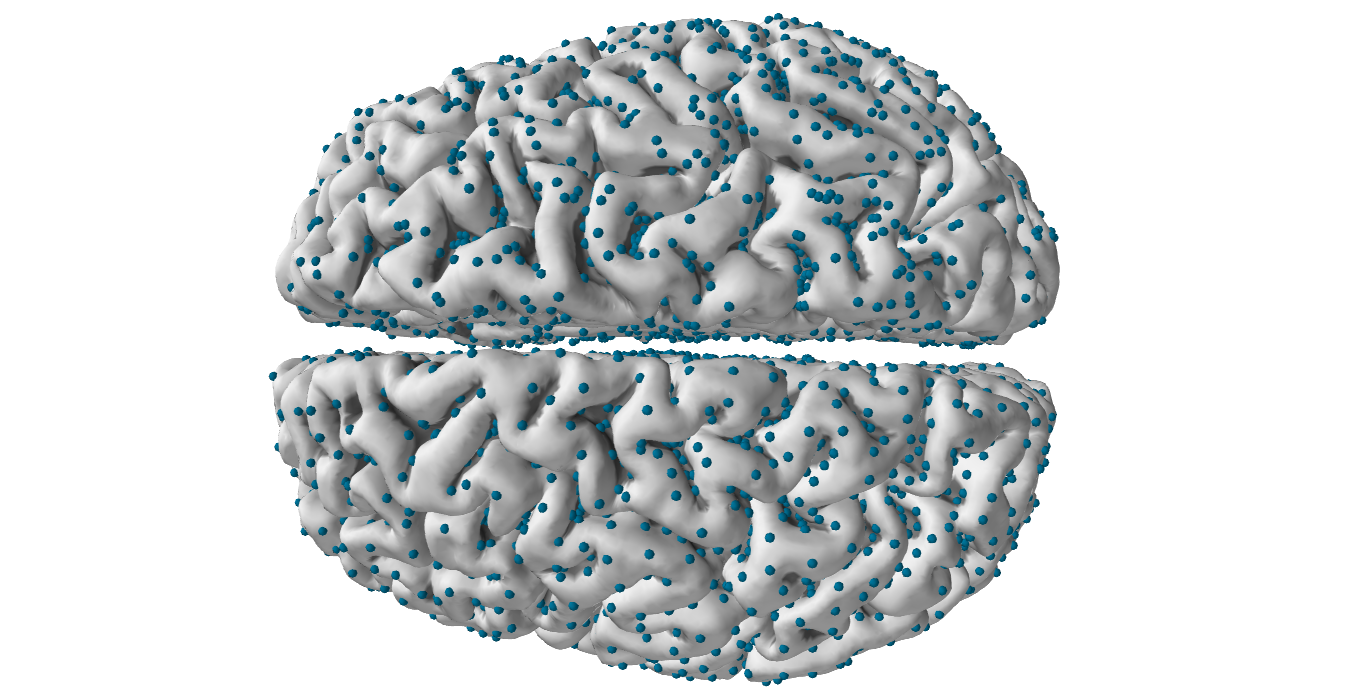
\includegraphics[scale=0.3]{../images/brain.png}
\caption{Пример сетки в пространстве источников,
          построенной на основе трехмерной анатомической модели}
\label{fig:src_space}
\end{figure}

\begin{equation}
    \mathbf{x}_k(t) = \mathbf{G} \cdot \mathbf{s}_k(t) + \mathbf{\omega}_k(t),
    \label{gm_ts}
\end{equation}
где $\mathbf{s}_k(t)$ --- $n$-мерный вектор-столбец активаций источников,
$\mathbf{x}_k(t)$ --- $m$-мерный вектор-столбец сигналов на сенсорах,
$t$ --- время, а $\mathbf{G}$ --- $m \times n$ матрица линейного отображения
пространства источников в пространство сенсоров.
Индекс $k$ обозначает номер эпохи.
Применим к (\ref{gm_ts}) частотное преобразование. Существует много способов произвести
эту операцию, например, --- вейвлет-преобразование или узкополосная фильтрация
с последующим аналитическим представлением сигнала.
Мы не будем вдаваться в подробности теории частотно-временных преобразований;
для подробного математизированного изложения предмета см.
\cite{Oppenheim1998}, о  применении  частотно-временных преобразований к обработке
электрофизиологических данных можно прочитать в \cite{Freeman}.
Мы только упомянем, что вне зависимости от особенностей выбранного
метода образом частотно-временного преобразования матрицы $\mathbf{X}$ размера $m \times T$
будет комплексный тензор, каждый временной срез которого содержит в себе информацию
о фазовом и амплитудном спектре сигнала в каждый момент времени.
Чтобы упростить вывод, мы зафиксируем одну частоту имея в виду,
что дальнейшие выкладки справедливы и для остальных частот преобразования. В итоге мы можем записать:

\begin{equation}
    \hat{\mathbf{x}}_{k,f_i}(t) = \mathbf{G} \cdot \hat{\mathbf{s}}_{k,f_i}(t) + \hat{\mathbf{\omega}}_{k,f_i}(t),
    \label{gm_timefreq}
\end{equation}
где $\hat{\mathbf{x}}, \hat{\mathbf{s}}, \hat{\mathbf{\omega}}$ --- комплекснозначные образы $\mathbf{x}, \mathbf{s}, \mathbf{\omega}$ соответственно.
Для простоты далее будем опускать нижний индекс $f_i$:

\begin{equation}
    \hat{\mathbf{x}}_k(t) = \mathbf{G} \cdot \hat{\mathbf{s}}_k(t) + \hat{\mathbf{\omega}}_k(t)
    \label{gm_timefreq_no_fi}
\end{equation}

\subsection{Порождающая модель матрицы кросс-спектральной плотности и метод ImCoh}
\label{sec:imcoh}
Теперь, если мы для каждой эпохи умножим $\hat{\mathbf{x}}_k(t)$ на его эрмитово сопряжение и усредним результат,
мы получим порождающую модель кросс-спектра на сенсорах:

\begin{gather}
           \langle{\hat{\mathbf{x}}_k(t) \hat{\mathbf{x}}_k(t)^{\dag}} \rangle_{k=1}^K =
           \langle{(\mathbf{G} \cdot\hat{\mathbf{s}}_k(t) + \hat{\mathbf{\omega}}_k(t))
                                       (\mathbf{G} \cdot\hat{\mathbf{s}}_k(t) + \hat{\mathbf{\omega}}_k(t))^{\dag}}\rangle_{k=1}^K=\nonumber\\
= \mathbf{G}  \cdot \langle{\hat{\mathbf{s     }}_k(t) \hat{\mathbf{s     }}_k(t)^{\dag}} \rangle_{k=1}^K \cdot \mathbf{G}^T +
   \mathbf{G} \cdot \langle{\hat{\mathbf{s     }}_k(t) \hat{\mathbf{\omega}}_k(t)^{\dag}} \rangle_{k=1}^K + \nonumber\\
        +  \langle{\hat{\mathbf{\omega}}_k(t) \hat{\mathbf{s     }}_k(t)^{\dag}} \rangle_{k=1}^K \cdot \mathbf{G}^T +
           \langle{\hat{\mathbf{\omega}}_k(t) \hat{\mathbf{\omega}}_k(t)^{\dag}} \rangle_{k=1}^K,
    \label{gm_cp_ini}
\end{gather}
\\
где оператор $\langle \cdot \rangle_{k=1}^K$ означает усреднение по эпохам.

Так как шум предполагается белым, а сигнал на сенсорах $\hat{\mathbf{s}}_k$ и шум $\hat{\mathbf{\omega}}_k$ взаимно независимыми,
можем заметить, что второй и третий члены уравнения (\ref{gm_cp_ini}) равны нулю, когда число эпох достаточно велико.
Также отметим, что
$\hat{\mathbf{x     }}_k(t) \hat{\mathbf{x     }}_k(t)^{\dag}$,
$\hat{\mathbf{s     }}_k(t) \hat{\mathbf{s     }}_k(t)^{\dag}$ и
$\hat{\mathbf{\omega}}_k(t) \hat{\mathbf{\omega}}_k(t)^{\dag}$
представляют собой внешние произведения комплексно-значных векторов на свои комплексные сопряжения,
и следовательно являются эрмитовыми матрицами, что означает,
что значения, находящиеся на диагоналях этих матриц, принадлежат к области вещественных чисел.
Это свойство, очевидно, сохраняется и после усреднения.
Более того, раз элементы векторов являются комплексными числами, они могут быть представлены в виде
$\hat{\xi}(t) = r(t)\cdot e^{i\phi(t)}$, где $\phi(t)$ соответствует мгновенной фазе сигнала,
а $r(t)$ амплитуде. Следовательно,
$\langle \hat{\xi}_p \hat{\xi}_q^* \rangle = \langle r_p r_q e^{i\Delta\phi} \rangle$ или,
если для иллюстрации мы примем, что амплитуды и фазы независимы
(справедливость последнего является предметом разногласий для электрофизиологических данных \cite{Lachaux1999}, \cite{imcoh}),
мы получим, что
$\langle \hat{\xi}_p \hat{\xi}_q^* \rangle = \langle r_p r_q \rangle \langle e^{i\Delta\phi} \rangle$.

Из последнего соотношения можно сделать несколько выводов.
Во-первых, элементы матрицы кросс-спектра представляют собой степень стабильности
разности фаз $\Delta\phi$ по эпохам.
Так, если разность фаз была достаточно равномерно распределена по всему возможному
интервалу принимаемых значений, то среднее $\langle e^{i\Delta\phi} \rangle$
будет приблизительно равно нулю.
С другой стороны, если разность фаз сохраняется от эпохи к эпохе,
результирующий коэффициент будет отличен от нуля,
что соответствует случаю установления коннективности между сигналами.
Во-вторых, если разность фаз мала,
элементы взаимного спектра могут быть близки к ненулевому вещественному числу.

Введем следующее обозначение для матрицы кросс-спектральной плотности:

\begin{equation}
    \Cp{v} \stackrel{def}{=} \langle{\hat{\mathbf{v}}_k(t) \hat{\mathbf{v}}_k(t)^{\dag}}\rangle_{k=1}^K, \\
    \label{cp_def}
\end{equation}
Используя определение (\ref{cp_def}) и опуская нулевые члены, (\ref{gm_cp_ini})
перепишется в виде
\begin{equation}
    \Cp{x}(t) = \mathbf{G} \Cp{s}(t) \mathbf{G}^T + \Cp{\omega}(t)
    \label{gm_cp_matr}
\end{equation}

Теперь рассмотрим более детально диагональ матрицы $\Cp{s}$.
Как уже было сказано, элементы главной диагонали этой матрицы являются вещественными числами
и они представляют собой значения мощностей сигналов пространства источников,
имеющих частоту $f_i$. В структуре порождающей модели отражен тот факт,
что после отображения оператором из пространства источников в пространство сенсоров
с помощью оператора $\mathbf{G}$ эти мощностные члены будут смешаны с истинной коннективностью,
и так как исходная система уравнений была сильно недоопределена (условие $n >> m$),
разделить сигналы не представляется возможным.
Математически, этим и объясняется эффект протечки сигнала.

Чтобы внести дополнительную ясность, представим себе ситуацию,
когда синхронизация между источниками полностью отсутствует,
но при этом некоторые участки мозга активны.
В такой постановке все элементы матрицы $\Cp{s}$, лежащие вне главной диагонали,
будут равны нулю, но для $\Cp{x}$ это выполняться не будет.
Пары сенсоров, расположенные близко к активным участкам мозга,
будут иметь большие кросс-спектральные коэффициенты,
что приведет к ложному обнаружению коннективности между источниками.

В ранее упомянутом методе ImCoh (в настоящее время, вероятно,
наиболее часто используемом для измерения коннективности)
предлагается рассматривать только мнимые части уравнения (\ref{gm_cp_matr}),
что уберегает нас от негативного эффекта протечки сигнала,
но при этом мы также теряем действительную часть <<хорошего>> сигнала, несущую
информацию о фазовой синхронизации.

\subsection{Оператор проецирования от протечки сигнала.}

Для более полного использования информации о фазовой синхронизации, содержащейся в кросс-спектре
мы предлагаем другой подход к устранению эффекта протечки сигнала.
Распишем  произведение матриц $\mathbf{G} \Cp{s} \mathbf{G}^T$ в правой части уравнения (\ref{gm_cp_matr}):

\begin{gather}
    \Cp{x}(t) = \sum\limits_{p=1}^n\sum\limits_{q=1}^n\mathbf{g}_p\mathbf{g}_q^T c_{pq}^{\mathbf{ss}}(t) + \Cp{\omega}(t),
    \label{cp_rhs_expanded}
\end{gather}
где $\mathbf{g}_p$ --- столбец матрицы $\mathbf{G}$, который называют \emph{топографией} источника $p$,
поскольку он определяет, каким образом сигнал, поступающий от источника $p$, будет виден на сенсорах.
Можно заметить, что кросс-спектр на уровне сенсоров представляет собой взвешенную сумму внешних произведений топографий,
взятую с коэффициентами, являющимися элементами кросс-спектра из пространства источников.

\subsection{Произведение Кронекера и векторизация}
Векторизуем уравнение (\ref{cp_rhs_expanded}):

\begin{gather}
    vec(\Cp{x}(t)) = \sum\limits_{p=1}^n\sum\limits_{q=1}^n vec(\mathbf{g}_p\mathbf{g}_q^T) c_{pq}^{\mathbf{ss}}(t) + vec(\Cp{\omega}(t))
    \label{cp_rhs_vec}
\end{gather}

Для упрощения записи будем использовать понятие произведения Кронекера.
Произведением Кронекера матриц $A$ и $B$, имеющих размеры $p\times q$ и $r\times s$ соответственно, называется матрица вида

\begin{equation}
    \mathbf{A} \otimes \mathbf{B} \stackrel{def}{=}
    \begin{bmatrix}
        a_{11} \mathbf{B} & a_{12} \mathbf{B} & \dots & a_{1n} \mathbf{B} \\
        a_{21} \mathbf{B} & a_{22} \mathbf{B} & \dots & a_{2n} \mathbf{B} \\
        \vdots            & \vdots            & \dots & \vdots            \\
        a_{m1} \mathbf{B} & a_{m2} \mathbf{B} & \dots & a_{mn} \mathbf{B}
        \label{kron_def}
     \end{bmatrix}
\end{equation}

Произведение Кронекера является билинейной ассоциативной операцией:

\begin{gather}
     \mathbf{A} \otimes (\mathbf{B} + \mathbf{C}) = \mathbf{A} \otimes \mathbf{B} + \mathbf{A} \otimes \mathbf{C} \\
    (\mathbf{A} + \mathbf{B}) \otimes \mathbf{C} = \mathbf{A} \otimes \mathbf{C} + \mathbf{B} \otimes \mathbf{C} \\
    \alpha(\mathbf{A} \otimes \mathbf{B}) = (\alpha\mathbf{A}) \otimes \mathbf{B} = \mathbf{A} \otimes (\alpha\mathbf{B}) \\
    \mathbf{A} \otimes(\mathbf{B} \otimes \mathbf{C}) =
   (\mathbf{A} \otimes \mathbf{B})\otimes \mathbf{C} =
    \mathbf{A} \otimes \mathbf{B} \otimes \mathbf{C}
\end{gather}

Заметим также, что произведение Кронекера не является симметричным: $\mathbf{A} \otimes \mathbf{B} \neq \mathbf{B} \otimes \mathbf{A}$.
Приведем другие полезные соотношения:

\begin{gather}
    (\mathbf{A} \otimes \mathbf{B})^T = \mathbf{A}^T \otimes \mathbf{B}^T \\
    (\mathbf{A} \otimes \mathbf{B}) (\mathbf{C} \otimes \mathbf{D}) = (\mathbf{A} \mathbf{B}) \otimes (\mathbf{C} \mathbf{D})
\end{gather}

Отметим особенно интересное для нас свойство произведения Кронекера, связывающее его с процедурой векторизации.
Для матриц $\mathbf{A}$, $\mathbf{B}$, $\mathbf{C}$ справедливо (доказательство см. в [10]):

\begin{equation}
    vec(\mathbf{A} \mathbf{B} \mathbf{C}) = (\mathbf{C}^T \otimes \mathbf{A}) vec(\mathbf{B})
    \label{eq:kron_vec}
\end{equation}

В нашем случае приведенное выражение принимает самую простую форму:

\begin{gather}
    vec[\mathbf{g}_p \mathbf{g}_q^T] = vec\left[
        \begin{pmatrix}
            g_p^1 \\
            \vdots \\
            g_p^m
        \end{pmatrix}
    \cdot 1 \cdot
    \begin{pmatrix}
        g_q^1 & \dots & g_q^m
    \end{pmatrix}
    \right] = %\nonumber \\
    \begin{pmatrix}
        g_q^1 \\
        \vdots \\
        g_q^m
    \end{pmatrix}
    \otimes
    \begin{pmatrix}
        g_p^1 \\
        \vdots \\
        g_p^m
    \end{pmatrix}
    \cdot
    vec(1) =
    \mathbf{g}_q \otimes \mathbf{g}_p,
\end{gather}


где $\mathbf{g}_q \otimes \mathbf{g}_p$ представляет собой вектор-столбец размера $m^2 \times 1$.
Введем понятие \emph{коммутационной матрицы} \cite{neudecker}.
Коммутационная матрица --- это матрица, которая связвает операции транспонирования и векторизации
и определяется следующим соотношением:

\begin{equation}
    vec(\mathbf{A}) = \mathbf{K}^{(m,n)} vec(\mathbf{A}^T)
    \label{eq:commutation_matrix_def}
\end{equation}
где $\mathbf{A}$~--- матрица размером $m \times n$, а матрица $\mathbf{K}^{(m,n)}$ имеет размеры
$mn \times mn$.
Матрица $K^{(m,n)}$ является частным случаем матрицы перестановок и
может быть получена из единичной перестановкой строк.

Далее нас будет интересовать только случай квадратных матриц $\mathbf{A}$.
Получим в явном виде выражение для коммутационной матрицы в случае квадратных матриц.

Пусть матрица $\mathbf{A}$ имеет размеры $n \times n$. Обозначим соответствующую ей коммутационную матрицу
как $\mathbf{K}_n$
Обозначим символом $\mathbf{e}_i$ вектор-столбец длины $n$, у которого на $i$-ом месте стоит
единица, а на всех остальных --- нули. Тогда для векторизации $\mathbf{A}^T$ будем иметь:

\begin{multline}
    vec\left(\mathbf{A}^T\right) = vec\left(\sum_{i,j} A_{i,j} \mathbf{e}_j \mathbf{e}_i^T\right) =
    vec\left(\sum_{i,j} (\mathbf{e}_i^T \mathbf{A} \mathbf{e}_j)(\mathbf{e}_j \mathbf{e}_i^T)\right) = \\
  = vec\left(\sum_{i,j} \mathbf{e}_j \mathbf{e}_i^T \mathbf{A} \mathbf{e}_j\mathbf{e}_i^T\right) =
    \sum_{i,j} vec\left(\mathbf{e}_j \mathbf{e}_i^T \mathbf{A} \mathbf{e}_j \mathbf{e}_i^T\right) =
    \left(\sum_{i,j} (\mathbf{e}_i \mathbf{e}_j^T) \otimes (\mathbf{e}_j \mathbf{e}_i^T) \right)vec(\mathbf{A})
\end{multline}

Таким образом,
\begin{equation}
    \mathbf{K}_n =  \sum_{i,j} (\mathbf{e}_i \mathbf{e}_j^T) \otimes (\mathbf{e}_j \mathbf{e}_i^T)
    \label{eq:commutation_matrix_formula}
\end{equation}

Теперь перепишем выражение (\ref{cp_rhs_vec}), используя новые обозначения:

\begin{equation}
    vec(\Cp{x}(t)) = \sum\limits_{p=1}^n\sum\limits_{q=1}^n
    \mathbf{g}_q\otimes \mathbf{g}_p \cdot c_{pq}^{\mathbf{ss}}(t) + vec(\Cp{\omega}(t))
    \label{cp_rhs_kron}
\end{equation}
Теперь можно видеть, что векторизованный кросс-спектр на уровне сенсоров представлен линейной
комбинацией векторов $\mathbf{g}_q \otimes \mathbf{g}_p$ в $m^2$-мерном векторном пространстве.
Назовем эти векторы \emph{2-топографиями}.
Нам уже известно, что эффект протечки сигнала, от которого необходимо избавиться,
обусловлен 2-топографиями особого вида $\mathbf{g}_p \otimes \mathbf{g}_p$ (всего $n$ векторов),
конкретный вид которых нам задан через оператор $\mathbf{G}$.
Следовательно, мы можем спроецировать выражение (\ref{cp_rhs_kron}) ортогонально линейному пространству,
натянутому на 2-топографии источников протечки сигнала.

\subsection{Построение оператора проецирования}
\label{sec:psiicos_projection}
Прежде чем мы начнем построение оператора ортогональной проекции от подпространства протечки сигнала,
необходимо понять, как соотносится подпространство протечки сигнала с линейными оболочками
2-топографий действительной и мнимой частей порождающей модели кросс-спектра на сенсорах.

Во-первых, выделим в уравнении (\ref{cp_rhs_kron}) действительную и мнимую части.
Заметим, что так как матрица $\Cp{s}$ является эрмитовой,
$c^{\mathbf{ss}}_{pq} = \overline{c^{\mathbf{ss}}_{qp}}$ (верхняя черта обозначает комплексное сопряжение):

\begin{gather}
    \sum\limits_{p=1}^n\sum\limits_{q=1}^n \mathbf{g}_q\otimes \mathbf{g}_p \cdot c_{pq}^{\mathbf{ss}}(t) =
    Re\left(\sum\limits_{p,q=1}^{n,n} \mathbf{g}_q\otimes \mathbf{g}_p \cdot c_{pq}^{\mathbf{ss}}(t)\right) +
     i \cdot Im\left(\sum\limits_{p,q=1}^{n,n}
     \mathbf{g}_q\otimes \mathbf{g}_p \cdot c_{pq}^{\mathbf{ss}}(t)\right) = \nonumber \\
           = \sum\limits_{p\leq q}^{n,n} (\mathbf{g}_q\otimes \mathbf{g}_p + \mathbf{g}_p\otimes \mathbf{g}_q)
           Re\left(c_{pq}^{\mathbf{ss}}(t)\right) +
     i \cdot \sum\limits_{p<q}^{n,n} (\mathbf{g}_q\otimes \mathbf{g}_p - \mathbf{g}_p\otimes \mathbf{g}_q)
           Im\left(c_{pq}^{\mathbf{ss}}(t)\right)
    \label{eq:cp_re_im}
\end{gather}

Отметим изменения в индексах суммирования.

Для удобства обозначим линейное пространство, натянутое на 2-топографии, ответственные за протечку сигнала, как
$S_{SL}$, а линейную оболочку 2-топографий мнимой части --- $S_{Im}$.

Из уравнения (\ref{eq:cp_re_im}) видно, что 2-топографии действительной и мнимой частей устроены по-разному,
а именно, --- векторы $\mathbf{g}_q \otimes \mathbf{g}_p + \mathbf{g}_p \otimes \mathbf{g}_q$
являются симметричными, тогда как 2-топографии мнимых частей
$\mathbf{g}_q \otimes \mathbf{g}_p - \mathbf{g}_p \otimes \mathbf{g}_q$ антисимметричны по индексам $p, q$.
Нас интересует, как это структурное отличие проявляется во взаимосвязи подпространств $S_{Re}$ и $S_{Im}$ с
подпространством протечки сигнала $S_{VC}$.
Покажем, что  2-топографии мнимой части ортогональны векторам,
на которые натянуто подпространство объемной проводимости:
\begin{gather}
    (\mathbf{g}_s \otimes \mathbf{g}_s)^T(\mathbf{g}_q \otimes \mathbf{g}_p - \mathbf{g}_p \otimes \mathbf{g}_q) =
        (\mathbf{g}_s^T \otimes \mathbf{g}_s^T)(\mathbf{g}_q \otimes \mathbf{g}_p) -
        (\mathbf{g}_s^T \otimes \mathbf{g}_s^T)(\mathbf{g}_p \otimes \mathbf{g}_q) = \nonumber \\
       =(\mathbf{g}_s^T \mathbf{g}_q \otimes \mathbf{g}_s^T \mathbf{g}_p -
         \mathbf{g}_s^T \mathbf{g}_p \otimes \mathbf{g}_s^T \mathbf{g}_q) \stackrel{*}{=}
        (\mathbf{g}_s^T \mathbf{g}_p \mathbf{g}_s^T \mathbf{g}_q -
         \mathbf{g}_s^T \mathbf{g}_p \mathbf{g}_s^T \mathbf{g}_q) = 0
         \label{eq:vc_ort_im}
\end{gather}

Равенство $*$ сохраняется, так как $\mathbf{g}^T_s \mathbf{g}_q$ и $\mathbf{g}_s^T \mathbf{g}_p$
являются скалярными величинами, и мы можем опустить операцию ``$\otimes$'' и поменять местами множители.
Из (\ref{eq:vc_ort_im}) можно видеть,
что подпространство объемной проводимости ортогонально мнимой части подпространства.
Для действительной части такое соотношение не сохраняется:
\begin{gather}
    (\mathbf{g}_s \otimes \mathbf{g}_s)^T(\mathbf{g}_q \otimes \mathbf{g}_p + \mathbf{g}_p \otimes \mathbf{g}_q) =
        (\mathbf{g}_s^T \otimes \mathbf{g}_s^T)(\mathbf{g}_q \otimes \mathbf{g}_p) +
        (\mathbf{g}_s^T \otimes \mathbf{g}_s^T)(\mathbf{g}_p \otimes \mathbf{g}_q) = \nonumber \\
       =(\mathbf{g}_s^T \mathbf{g}_q \otimes \mathbf{g}_s^T \mathbf{g}_p +
         \mathbf{g}_s^T \mathbf{g}_p \otimes \mathbf{g}_s^T \mathbf{g}_q) =
        2\langle\mathbf{g}_s, \mathbf{g}_p\rangle \langle\mathbf{g}_s, \mathbf{g}_q\rangle
         \label{eq:vc_ort_re}
\end{gather}

После проведенных операций легко увидеть, что проекция ортогонально подпространству протечки сигнала
оказывает влияние на подпространство действительной части кросс-спектра на источниках.
Следовательно, нужно добиться того, чтобы протечка сигнала была удалена из данных
насколько это возможно с учетом минимального воздействия на подпространство
действительной части кросс-спектра (см.рис.~\ref{fig:subspaces}).
Для достижения этой цели необходимо уменьшить размерность подпространства
объемной проводимости неким оптимальным способом.

\begin{figure}[htbp]
\centering
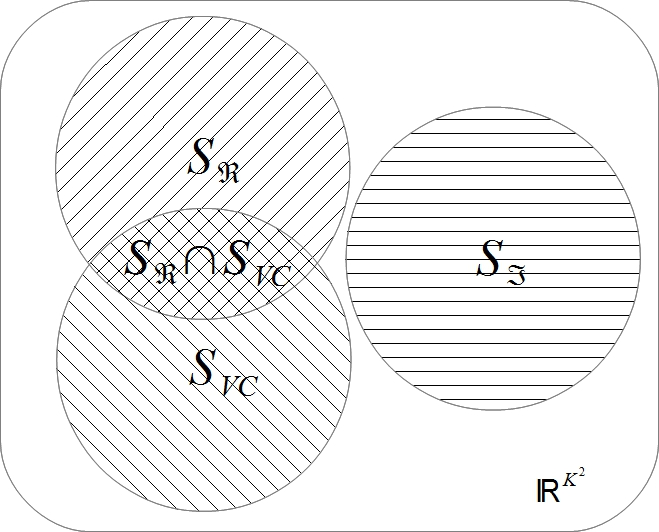
\includegraphics[width=12cm]{./images/SetsReImVC.jpg}
\caption{Взаимосвязь подпространств для кросс-спектра на уровне сенсоров}
\medskip
\small
Подпространство протечки сигнала $S_{SL}$ и подпространство действительной части кросс-спектра $S_{\Re}$
имеют непустое пересечение. Кроме того, оба этих подпространства ортогональны подпространству мнимой
части кросс-спектра $S_{\Im}$.
Пересечение $S_{SL}$ с $S_{\Re}$ содержит вклад как от протечки сигнала,
так и от истинно взаимодействующих источников,
расположенных близко друг к другу и характеризующихся малой разностью фаз.
\label{fig:subspaces}
\end{figure}%
Имея в виду все вышеперечисленное, вернемся к построению проектора.
Рассмотрим матрицу, составленную из вектор-столбцов, образующих подпространство протечки сигнала:

\begin{equation}
    \mathbf{F} =
    \begin{bmatrix}
        |                                 & |                                 &       & |                                 \\
        \mathbf{g}_1 \otimes \mathbf{g}_1 & \mathbf{g}_2 \otimes \mathbf{g}_2 & \dots & \mathbf{g}_n \otimes \mathbf{g}_n \\
        |                                 & |                                 &       & |
    \end{bmatrix}
\end{equation}

Произведем сингулярное разложение матрицы $\mathbf{F}$ \cite{Golub1996}.

\begin{equation}
    \mathbf{F} = \mathbf{USV}^T
    =
    \begin{bmatrix}
        |            & |            &        & |       \\
        \mathbf{u}_1 & \mathbf{u}_2 & \dots  & \mathbf{u}_{m^2} \\
        |            & |            &        & |
    \end{bmatrix}
    % S
    % \begin{pmatrix}
    %   \lambda_1 & 0         & \dots   & 0             & 0 & \dots & 0 \\
    %   0         & \lambda_2 & \dots   & \vdots        & 0 & \dots & 0 \\
    %   \vdots    &           & \ddots  & 0             & 0 & \dots & 0 \\
    %   0         & \dots     & \dots   & \lambda_{m^2} & 0 & \dots & 0
    % \end{pmatrix}
    \begin{pmatrix}
        \lambda_1 & 0         & \dots    \\
        0         & \lambda_2 & \dots    \\
        \vdots    &           & \ddots
    \end{pmatrix}
    % Diag(\lambda_1, \dots, \lambda_{m^2})
    \begin{bmatrix}
        - & \mathbf{v}_1 & - \\
        - & \mathbf{v}_2 & - \\
          & \dots        &   \\
        - & \mathbf{v}_n & -
    \end{bmatrix}
    \label{eq:svd_f_fixed_or}
\end{equation}
\\
В соответствии со свойствами сингулярного разложения, первые $r$ колонок матрицы $\mathbf{U}$
образуют ортонормальный базис $r$-мерного линейного пространства,
являющегося лучшим $r$-мерным приближением $n$-мерного
подпространства протечки сигнала. Используем эти $r$ векторов для построения проектора с уменьшенным рангом:

\begin{gather}
    \mathbf{U}_r =
    \begin{bmatrix}
        |            & |            &        & |       \\
        \mathbf{u}_1 & \mathbf{u}_2 & \dots  & \mathbf{u}_r \\
        |            & |            &        & |
    \end{bmatrix}\label{eq:U_fixed_or};\\
    \mathbf{P}_r = \mathbf{I} - \mathbf{U}_r \mathbf{U}_r^T\label{eq:P_fixed_or}
 \end{gather}

Итак, мы построили оператор проекции ортогонально подпространству протечки сигнала $\mathbf{P}_r$
с сокращенным рангом $r$.
Умножение уравнения (\ref{cp_rhs_kron}) на этот оператор приводит к тому, что  из порождающей
модели кросс-спектра на уровне сенсоров частично удаляются члены ответственные за эффект протечки сигнала;
параметр $r$ при этом определяет баланс между желаемым уровнем очистки от протечки сигнала и
воздействием проектора на действительную часть кросс-спектра.

Окончательно, выражение для кросс-спектра на уровне сенсоров после проекции от протечки сигнала
запишется в виде:

\begin{equation}
    vec(\Cp{x})^\perp = \mathbf{P}_r vec(\Cp{x}) =
    \sum\limits_{p=1}^n\sum\limits_{q=1}^n \mathbf{P}_r \mathbf{g}_q\otimes
    \mathbf{g}_p \cdot c_{pq}^{\mathbf{ss}}(t) + \mathbf{P}_r vec(\Cp{\omega}(t))
    \label{eq:cp_final}
\end{equation}

Или, пользуясь \ref{eq:cp_re_im}:
\begin{multline}
    vec(\Cp{x})^\perp = \sum\limits_{p\leq q}^{n,n}
    \mathbf{P}_r(\mathbf{g}_q\otimes \mathbf{g}_p + \mathbf{g}_p\otimes \mathbf{g}_q)
           Re\left(c_{pq}^{\mathbf{ss}}(t)\right) + \\
    + i \cdot \sum\limits_{p<q}^{n,n} (\mathbf{g}_q\otimes \mathbf{g}_p - \mathbf{g}_p\otimes \mathbf{g}_q)
           Im\left(c_{pq}^{\mathbf{ss}}(t)\right) +
           \mathbf{P}_r vec(\Cp{\omega}(t))
    \label{eq:cp_final_re_im}
\end{multline}

Отметим, что в мнимой части \ref{eq:cp_final_re_im} оператор проецирования $\mathbf{P}_r$ можно опустить
в силу \ref{eq:vc_ort_im}.

Элементы полученного таким образом векторизованного кросс-спектра $vec(\Cp{x})^\perp$ теперь могут быть
использованы для оценки коннективностей как на уровне сенсоров, так и в источниках.

\subsection{Модели со свободной ориентацией диполя}
С точки зрения анатомии каждая топография прямой модели $\mathbf{G}$
представляет собой распределение электромагнитного поля,
порождаемого так называемыми первичными токами, то есть токами,
текущими через апикальные дендриты кортикальных пирамидальных нейронов.
Так как апикальные дендриты расположены перпендикулярно к кортикальной мантии,
первичные токи по отношению к кортикальной мантии также имеют нормальную ориентацию.
Следовательно, точность прямой модели напрямую зависит от точности оценки вектора нормали
к поверхности коры, а значит и от количества точек, используемых для аппроксимации поверхности коры.
Вместе с тем, хотя современное моделирование с использованием метода магнитно-резонансной
томографии позволяет получать весьма детальную реконструкцию мозга с размером аппроксимирующих сеток
порядка нескольких сотен тысяч узлов, использование столь подробных сеток приводит к значительному
ухудшению производительности алгоритмов, работающих в пространстве источников, вследствие высоких затрат
по памяти и вычислительному времени при работе с большими массивами данных.

По этой причине использование разреженных сеток со сравнительно небольшим числом узлов стало
общепринятой практикой. Как уже отмечалось выше, недостаток такого подхода состоит в том, что
при прореживании сетки эффективная ориентация локальной нормали к коре становится неопределенной.

Неопределенность появляется из-за того, что после разрежения размер области на коре, соответствующей отдельно
взятому узлу сетки, возрастает, и так как каждая такая область характеризуется в общем случае
переменной кривизной, эффективная ориентация токового диполя,
находящегося внутри отдельно взятой области аппроксимации,
будет зависеть от того, в какой именно части области находился диполь в тот или иной момент записи.

Частично справиться с этим эффектом позволяют модели, со \emph{свободной ориентацей диполя},
в которых эффективная ориентация становится дополнительным параметром,
который необходимо оценить из данных~\cite{Lin2006}.

Для учета свободной ориентации следует представить топографию в точке $p$ коры в виде линейной
комбинации трех ортогональных друг к другу векторов топографии, размещенных в одной точке:
\begin{equation}
    \mathbf{g}_p = \mathbf{g}_p^x \xi + \mathbf{g}_p^y \eta + \mathbf{g}_p^z \zeta =
    [\mathbf{g}_p^x, \mathbf{g}_p^y, \mathbf{g}_p^z] \left(
    \begin{array}{ccc}
        \xi \\
        \eta \\
        \zeta
    \end{array}
    \right)
    \label{loose_or}
\end{equation}

В случае МЭГ измерений, для модели сферически симметричного проводника,
магнитное поле от токового диполя с радиальной ориентацией равно нулю, и следовательно
введенная тройка векторов может быть заменена парой диполей в плоскости,
перпендикулярной радиальному направлению для каждого узла.
Следовательно, уравнение (\ref{loose_or}) перепишется для МЭГ в виде

\begin{equation}
    \mathbf{g}_p = \mathbf{g}_p^x \xi + \mathbf{g}_p^y \eta = [\mathbf{g}_p^x, \mathbf{g}_p^y] \left(
    \begin{array}{ccc}
        \xi \\
        \eta
    \end{array}
    \right)
    \label{loose_or_meg}
\end{equation}

Соответственно изменятся выражения и для 2-топографий протечки сигнала:

\begin{gather}
    \mathbf{g}_p \otimes \mathbf{g}_p = (\mathbf{g}_p^x \xi
                                      + \mathbf{g}_p^y \eta) \otimes (\mathbf{g}_p^x \xi
                                      + \mathbf{g}_p^y \eta) = \nonumber \\
                                      = \mathbf{g}_p^x \otimes \mathbf{g}_p^x \xi^2
                                      + \mathbf{g}_p^x \otimes \mathbf{g}_p^y \xi \eta
                                      + \mathbf{g}_p^y\otimes  \mathbf{g}_p^x \eta \xi
                                      + \mathbf{g}_p^y \otimes \mathbf{g}_p^y \eta^2 = \nonumber \\
                                      = [\mathbf{g}_p^x \otimes \mathbf{g}_p^x,
                                         \mathbf{g}_p^x \otimes \mathbf{g}_p^y
                                      + \mathbf{g}_p^y \otimes \mathbf{g}_p^x,
                                        \mathbf{g}_p^y \otimes \mathbf{g}_p^y]
\left( \begin{array}{ccc}
\xi^2 \\
\xi \eta \\
\eta^2
\end{array}
\right)
\label{eq:orient_dip_comps}
\end{gather}

Выражение в квадратных скобках здесь представляет собой матрицу, записанную по столбцам.
Можно заметить,
что 2-топографии протечки сигнала теперь принадлежат линейной оболочке трех векторов,
а именно~---
$\mathbf{g}_p^x \otimes \mathbf{g}_p^x$, $\mathbf{g}_p^x \otimes \mathbf{g}_p^y +
\mathbf{g}_p^y \otimes \mathbf{g}_p^x$ и $\mathbf{g}_p^y \otimes \mathbf{g}_p^y$.
Разумеется, представленная таким образом 2-топография протечки сигнала зависит только от параметра
$\theta_p$ --- угла между эффективной ориентацией топографии $\mathbf{g}_p$ и ее $х$-компоненты~---
через $\xi = sin(\theta_p)$ и $\eta=cos(\theta_p)$:

\begin{equation*}
    \mathbf{g}_p \otimes \mathbf{g}_p =
    [\mathbf{g}_p^x \otimes \mathbf{g}_p^x, \mathbf{g}_p^x \otimes \mathbf{g}_p^y +
     \mathbf{g}_p^y \otimes \mathbf{g}_p^x, \mathbf{g}_p^y \otimes \mathbf{g}_p^y]
    \left( \begin{array}{ccc}
    cos(\theta_p)^2 \\
    cos(\theta_p) sin(\theta_p) \\
    sin(\theta_p)^2
    \end{array}
    \right)
\end{equation*}

Но это однопараметрическое семейство векторов не может быть эффективно сведено к линейному векторному
пространству с размерностью меньше 3 для построения соответствующего проектора,
а значит в случае МЭГ для модели сферически симметричного проводника мы должны добавить все три
2-топографии источника $p$ в матрицу $F$:

\begin{equation}
    \mathbf{F} =
    \begin{bmatrix}
        \mathbf{g}_1^x \otimes \mathbf{g}_1^x, &
        \mathbf{g}_1^x \otimes \mathbf{g}_1^y + \mathbf{g}_1^y \otimes \mathbf{g}_1^x, &
        \mathbf{g}_2^x \otimes \mathbf{g}_2^x, &
        \dots, & \mathbf{g}_n^y \otimes \mathbf{g}_n^y \\
    \end{bmatrix}
\end{equation}

Рассмотрим теперь случай ЭЭГ-измерений. Так как в случае ЭЭГ линейные подпространства, натянутые
на три вектора топографий в каждой точке, вообще говоря имеют разммерность 3, мы вынуждены
учитывать каждый из векторов топографий при составлении матрицы $\mathbf{F}$.
Тем не менее, расписав аналог выражения~\ref{eq:orient_dip_comps}
для свободно ориентированного диполя в случае ЭЭГ,
получим, что независимых векторов  в подпространстве объемной проводимости для источника с индексом $p$
будет всего 6 (вместо возможных 9):


\begin{multline}
    \mathbf{g}_p \otimes \mathbf{g}_p = (\mathbf{g}_p^x \xi
    + \mathbf{g}_p^y \eta
    + \mathbf{g}_p^z \zeta)
    \otimes
    (\mathbf{g}_p^x \xi
    + \mathbf{g}_p^y \eta
    + \mathbf{g}_p^z \zeta) =
    \nonumber \\
    = \mathbf{g}_p^x \otimes \mathbf{g}_p^x \xi^2
    + \mathbf{g}_p^y \otimes \mathbf{g}_p^y \eta^2
    + \mathbf{g}_p^z \otimes \mathbf{g}_p^z \zeta^2+\\
    + \mathbf{g}_p^x \otimes \mathbf{g}_p^y \xi \eta
    + \mathbf{g}_p^y\otimes  \mathbf{g}_p^x \eta \xi+\\
    + \mathbf{g}_p^x \otimes \mathbf{g}_p^z \xi \zeta
    + \mathbf{g}_p^z\otimes  \mathbf{g}_p^x \zeta \xi+\\
    + \mathbf{g}_p^y \otimes \mathbf{g}_p^z \eta \zeta
    + \mathbf{g}_p^z \otimes \mathbf{g}_p^y \zeta \eta
    =\\
    =  [\mathbf{g}_p^x \otimes \mathbf{g}_p^x,
        \mathbf{g}_p^y \otimes \mathbf{g}_p^y,
        \mathbf{g}_p^z \otimes \mathbf{g}_p^z,
        \mathbf{g}_p^x \otimes \mathbf{g}_p^y
        + \mathbf{g}_p^y \otimes \mathbf{g}_p^x,
        \mathbf{g}_p^x \otimes \mathbf{g}_p^z
        + \mathbf{g}_p^z \otimes \mathbf{g}_p^x,
        \mathbf{g}_p^y \otimes \mathbf{g}_p^z
        + \mathbf{g}_p^z \otimes \mathbf{g}_p^y]
        \left( \begin{array}{ccc}
                \xi^2 \\
                \eta^2 \\
                \zeta^2 \\
                \xi \eta \\
                \xi \zeta \\
                \eta \zeta
            \end{array}
        \right)
\end{multline}

Выражение в квадратных скобках вновь обозначает матрицу, записанную по столбцам,
а $\xi, \eta, \zeta$~--- компоненты разложения диполя с истинной ориентацией по базису
$\mathbf{g}_p^x,\mathbf{g}_p^y,\mathbf{g}_p^z$.

Все шесть колонок для каждого источника $p$ матрицы в выражении выше для ЭЭГ должны быть добавлены
в матрицу $\mathbf{F}$ для последующего расчета операции проецирования.

Повторяя далее процедуру \ref{eq:svd_f_fixed_or}, \ref{eq:U_fixed_or}, \ref{eq:P_fixed_or}, получим
оператор проекции от протечки сигнала в случае свободной ориентации диполя.

Рассмотрим теперь, как преобразуется уравнение \ref{eq:cp_final}
для свободной ориентации диполя в случае МЭГ и ЭЭГ.
Проведем рассуждения сначала для ЭЭГ, а затем упростим для случая сферической симметрии в МЭГ.

Итак, теперь векторы $\mathbf{g}_p, \mathbf{g}_q$ представляют собой
линейную комбинацию троек дипольных векторов $\mathbf{g}^x, \mathbf{g}^y, \mathbf{g}^z$.
Обозначим $\xi_p, \eta_p, \zeta_p$ значения проекций вектора $\mathbf{g}_p$ на
$\mathbf{g}_p^x, \mathbf{g}_p^y, \mathbf{g}_p^z$, для вектора $\mathbf{g}_q$ определим аналогичные величины
$\xi_q, \eta_q, \zeta_q$. Тогда для 2-топографии сети $p-q$, пользуясь \ref{eq:kron_vec} будем иметь:

\begin{multline}
    \mathbf{g}_p \otimes \mathbf{g}_q =
    vec\left(
        \begin{bmatrix}
            |              & |              & |              \\
            \mathbf{g}_p^x & \mathbf{g}_p^y & \mathbf{g}_p^z \\
            |              & |              & |
        \end{bmatrix}
        \left( \begin{array}{ccc}
                \xi_p \\
                \eta_p \\
                \zeta_p \\
            \end{array}
        \right)
        \left(\begin{array}{ccc}
                \xi_q,
                \eta_q,
                \zeta_q
            \end{array}
        \right)
        \begin{bmatrix}
            -             & \mathbf{g}_q^x & -   \\
            -             & \mathbf{g}_q^y & -   \\
            -             & \mathbf{g}_q^z & -
        \end{bmatrix}
    \right) = \\
  = \begin{bmatrix}
        |                 & |              & |              \\
        \mathbf{g}_q^x    & \mathbf{g}_q^y & \mathbf{g}_q^z \\
        |                 & |              & |
    \end{bmatrix}
    \otimes
    \begin{bmatrix}
        |                 & |              & |              \\
        \mathbf{g}_p^x    & \mathbf{g}_p^y & \mathbf{g}_p^z \\
        |                 & |              & |
    \end{bmatrix}
    \cdot
    \left(\begin{array}{ccc}
            \xi_q\\
            \eta_q\\
            \zeta_q
        \end{array}
    \right)
    \otimes
    \left(\begin{array}{ccc}
            \xi_p\\
            \eta_p\\
            \zeta_p
        \end{array}
    \right)
    \label{eq:kron_topo_free_or}
\end{multline}

Пользуясь выражением \ref{eq:kron_topo_free_or} рассмотрим, как будут устроены топографии
действительной и мнимой части для свободной ориентации диполя. Для компактности
обозначим тройку векторов топографий для диполя с индексом $k$ как $\mathbf{\mathbf{\Gamma}}_k$:

\begin{equation}
    \mathbf{\Gamma}_k =
    \begin{bmatrix}
        |                 & |              & |              \\
        \mathbf{g}_k^x    & \mathbf{g}_k^y & \mathbf{g}_k^z \\
        |                 & |              & |
    \end{bmatrix}
\end{equation}


Тогда для действительной части, пользуясь \ref{eq:commutation_matrix_formula}, получим:
\begin{multline}
    \mathbf{g}_p \otimes \mathbf{g}_q + \mathbf{g}_q \otimes \mathbf{g}_p = \\
    =
    \mathbf{\Gamma}_q
    \otimes
    \mathbf{\Gamma}_p
    \cdot
    \left(\begin{array}{ccc}
            \xi_q\\
            \eta_q\\
            \zeta_q
        \end{array}
    \right)
    \otimes
    \left(\begin{array}{ccc}
            \xi_p\\
            \eta_p\\
            \zeta_p
        \end{array}
    \right) +
    \mathbf{\Gamma}_p
    \otimes
    \mathbf{\Gamma}_q
    \cdot
    \left(\begin{array}{ccc}
            \xi_p\\
            \eta_p\\
            \zeta_p
        \end{array}
    \right)
    \otimes
    \left(\begin{array}{ccc}
            \xi_q\\
            \eta_q\\
            \zeta_q
        \end{array}
    \right) = \\
    =  \left(
        \mathbf{\Gamma}_q
    \otimes
    \mathbf{\Gamma}_p
  +
  \mathbf{\Gamma}_p
    \otimes
    \mathbf{\Gamma}_q
    \cdot
    \mathbf{K}_3
    \right)
    \cdot
    % \cdot
    \left(\begin{array}{ccc}
            \xi_q\\
            \eta_q\\
            \zeta_q
        \end{array}
    \right)
    \otimes
    \left(\begin{array}{ccc}
            \xi_p\\
            \eta_p\\
            \zeta_p
        \end{array}
    \right)
\end{multline}

В последнем равенстве мы поменяли порядок сомножителей в произведении Кронекера
векторов $(\xi,\eta,\zeta)^T$. Здесь $\mathbf{K}_3$~--- матрица коммутации,
определенная в соответствии с \ref{eq:commutation_matrix_def}.
В явном виде матрица $K_3$ в соответствии с формулой  \ref{eq:commutation_matrix_formula}
запишется как:
\begin{equation}
    \renewcommand{\arraystretch}{0.8}
    \mathbf{K}_3 =
    \begin{bmatrix}
        \textcolor{red}{1} & 0 & 0 & 0 & 0 & 0 & 0 & 0 & 0 \\
        0 & 0 & 0 & \textcolor{red}{1} & 0 & 0 & 0 & 0 & 0 \\
        0 & 0 & 0 & 0 & 0 & 0 & \textcolor{red}{1} & 0 & 0 \\
        0 & \textcolor{red}{1} & 0 & 0 & 0 & 0 & 0 & 0 & 0 \\
        0 & 0 & 0 & 0 & \textcolor{red}{1} & 0 & 0 & 0 & 0 \\
        0 & 0 & 0 & 0 & 0 & 0 & 0 & \textcolor{red}{1} & 0 \\
        0 & 0 & \textcolor{red}{1} & 0 & 0 & 0 & 0 & 0 & 0 \\
        0 & 0 & 0 & 0 & 0 & \textcolor{red}{1} & 0 & 0 & 0 \\
        0 & 0 & 0 & 0 & 0 & 0 & 0 & 0 & \textcolor{red}{1}
    \end{bmatrix}
\end{equation}


Аналогично для 2-топографий мнимой части будем иметь:
\begin{multline}
    \mathbf{g}_p \otimes \mathbf{g}_q - \mathbf{g}_q \otimes \mathbf{g}_p = \\
    =
    \mathbf{\Gamma}_q
    \otimes
    \mathbf{\Gamma}_p
    \cdot
    \left(\begin{array}{ccc}
            \xi_q\\
            \eta_q\\
            \zeta_q
        \end{array}
    \right)
    \otimes
    \left(\begin{array}{ccc}
            \xi_p\\
            \eta_p\\
            \zeta_p
        \end{array}
    \right) -
    \mathbf{\Gamma}_p
    \otimes
    \mathbf{\Gamma}_q
    \cdot
    \left(\begin{array}{ccc}
            \xi_p\\
            \eta_p\\
            \zeta_p
        \end{array}
    \right)
    \otimes
    \left(\begin{array}{ccc}
            \xi_q\\
            \eta_q\\
            \zeta_q
        \end{array}
    \right) = \\
    =  \left(
        \mathbf{\Gamma}_q
    \otimes
    \mathbf{\Gamma}_p
  -
  \mathbf{\Gamma}_p
    \otimes
    \mathbf{\Gamma}_q
    \cdot
    \mathbf{K}_3
    \right)
    \cdot
    % \cdot
    \left(\begin{array}{ccc}
            \xi_q\\
            \eta_q\\
            \zeta_q
        \end{array}
    \right)
    \otimes
    \left(\begin{array}{ccc}
            \xi_p\\
            \eta_p\\
            \zeta_p
        \end{array}
    \right)
\end{multline}

Для МЭГ в случае сферической симметрии соответствующие формулы будут выглядеть как
\begin{gather}
    \mathbf{g}_p \otimes \mathbf{g}_q + \mathbf{g}_q \otimes \mathbf{g}_p =
    \left(
        \mathbf{\Gamma}_q
        \otimes
        \mathbf{\Gamma}_p
        +
        \mathbf{\Gamma}_p
        \otimes
        \mathbf{\Gamma}_q
        \cdot
        \mathbf{K}_2
    \right)
    \cdot
    % \cdot
    \left(\begin{array}{ccc}
            \xi_q\\
            \eta_q\\
        \end{array}
    \right)
    \otimes
    \left(\begin{array}{ccc}
            \xi_p\\
            \eta_p\\
        \end{array}
    \right) \\
    \mathbf{g}_p \otimes \mathbf{g}_q - \mathbf{g}_q \otimes \mathbf{g}_p =
    \left(
        \mathbf{\Gamma}_q
        \otimes
        \mathbf{\Gamma}_p
        -
        \mathbf{\Gamma}_p
        \otimes
        \mathbf{\Gamma}_q
        \cdot
        \mathbf{K}_2
    \right)
    \cdot
    % \cdot
    \left(\begin{array}{ccc}
            \xi_q\\
            \eta_q\\
        \end{array}
    \right)
    \otimes
    \left(\begin{array}{ccc}
            \xi_p\\
            \eta_p\\
        \end{array}
    \right) \\
    \renewcommand{\arraystretch}{0.8}
    \mathbf{K}_2 =
    \begin{bmatrix}
        \textcolor{red}{1} & 0 & 0 & 0 \\
        0 & 0 & \textcolor{red}{1} & 0 \\
        0 & \textcolor{red}{1} & 0 & 0 \\
        0 & 0 & 0 & \textcolor{red}{1}
    \end{bmatrix}
\end{gather}

Окончательно выражение формула \ref{eq:cp_final_re_im} для ЭЭГ и
сферически-симметричного случая МЭГ запишется как

\begin{multline}
    vec(\Cp{x})^\perp = \sum\limits_{p\leq q}^{n,n}
    \mathbf{P}_r(\mathbf{\Gamma}_q\otimes \mathbf{\Gamma}_p +
                 \mathbf{\Gamma}_p\otimes \mathbf{\Gamma}_q\cdot \mathbf{K}_l)
                 \mathbf{\theta}_q \otimes \mathbf{\theta}_p
           Re\left(c_{pq}^{\mathbf{ss}}(t)\right) + \\
       +    i \cdot \sum\limits_{p<q}^{n,n}
           (\mathbf{\Gamma}_q\otimes \mathbf{\Gamma}_p -
            \mathbf{\Gamma}_p\otimes \mathbf{\Gamma}_q\cdot \mathbf{K}_l)
            \mathbf{\theta}_q \otimes \mathbf{\theta}_p
           Im\left(c_{pq}^{\mathbf{ss}}(t)\right) + \\
       +   \mathbf{P}_r vec(\Cp{\omega}(t))
    \label{eq:cp_final_re_im_free_or}
\end{multline}
где $l=2$ для МЭГ и $l=3$ для ЭЭГ, а $\mathbf{\theta}_k$ -- двухмерный или трехмерный вектор ориентации токового диполя.

Уравнение \ref{eq:cp_final_re_im_free_or} послужит нам отпревной точкой для дальнейшего анализа.
Далее из него необходимо оценить комплексные коэффициенты матрицы кросс-спектральной плотности мощности в
пространстве источников, а также неизвестные вектора ориентаций $\mathbf{\theta}_k$.
%\newpage
%========================================================================================================

